% Copyright FG Mauthe, University of Koblenz-Landau, Koblenz, Germany
% v1.0, last changed 19.04.21

\documentclass[%
	BCOR=8mm, % Bindekorrektur
	DIV=12, 
	toc=bibliography, % references in contents
	toc=listof, % list of tables and figures in contents
	oneside, %use twoside if preferred
	egregdoesnotlikesansseriftitles, % deletes the usage of sffamily font
	]{scrbook}

% Set the font right away, this is global, egregdoesnotlikesansseriftitles is already set, but overwritten with this command
\renewcommand{\familydefault}{\sfdefault} % bfseries

% Alternative, needs to be adjusted
%\documentclass[a4paper, twoside]{article}

%\newlength{\laenge}
%\setlength{\laenge}{2mm}
%\setlength{\parindent}{2\laenge}

\usepackage{xcolor}
\pagecolor{white} % white pages

% Font / Formatting packages
\usepackage[latin1]{inputenc}   % font-coding
\usepackage{listingsutf8}
\usepackage{caption}
\usepackage{subfigure}
\usepackage{cite}
\usepackage{lmodern}
\usepackage{multirow}
% Use either English or German 
\usepackage[english]{babel} 
%\usepackage[ngerman]{babel} 

% Math packages
\usepackage{amsmath} % math package
\usepackage{amsfonts} % for additional mathematical symbols
\usepackage{dsfont} % double stroke fonts, for instance to depict the natural numbers symbol |N

% More useful packages
\usepackage{float} % for "containers"
\usepackage{url}
\usepackage[onehalfspacing]{setspace} % simple option to change the spacing
\usepackage{layout}
\usepackage{fancyhdr}	% header
\usepackage{graphicx} 
\usepackage{booktabs} % For prettier tables
\usepackage{chngcntr} % enables the additional numbering of figures and tables
\usepackage{hyperref} % for clickable and marked cross references
%\usepackage{pdfpages}
\usepackage{forest}


% APPENDIX
\usepackage[toc,page]{appendix} % in case you'd like to use an appendix

\begin{document}

% Title Page
% Copyright FG Mauthe, University of Koblenz-Landau, Koblenz, Germany
% Apply the necessary changes to make this page your own

\begin{titlepage}
	
\includegraphics[height=35pt]{img/uni-logo.png}
	\hfill
	
\includegraphics[height=35pt]{img/iwvi.jpg}

	\begin{center}
	\vspace{2.5cm}	
	
	\huge\textbf{Assessment of Mean Teacher and Prominent Adversarial Unlabeled Data for Language Classification}
	
	%\vspace{2cm}


	\normalsize
	\vspace{1.5cm}	

	\textsc{\Large Masterarbeit}\\Master of Science (M.Sc.) im Web and Data Science\\[2cm] 
		
	vorgelegt von\\
	
	\textbf{\Large Bhupender Kumar Saini}\\ $ [ $219 100 887$ ] $\\ [1.5cm] 
	
	Koblenz, im February 2022
	\end{center}
	\vfill
	\begin{tabular}{ll}
		Erstgutachter: & Prof. Dr. Andreas Mauthe\\ 
		 & \small{(Institut f\"ur Wirtschafts- und Verwaltungsinformatik, FG Mauthe)}\\
		Zweitgutachter: & Alexander Rosenbaum, M. Sc. \\ 
		& \small{(Institut f\"ur Wirtschafts- und Verwaltungsinformatik, FG Mauthe)}\\
		%Ggf. ext. Betreuer eintragen.
		%Betreuer:  & Max Mustermann, M.Sc.
	\end{tabular}
\end{titlepage}


% Student's declaration
% Copyright FG Mauthe, University of Koblenz-Landau, Koblenz, Germany

% Declaration
% ===> Do NOT CHANGE anything here

\pagestyle{empty}
\begin{quote}
	\textbf{\Large Eidesstattliche Erkl\"arung}

	Ich versichere, dass ich die vorliegende Arbeit selbst\"andig verfasst
	und keine anderen als die angegebenen Quellen und Hilfsmittel benutzt habe
	und dass die Arbeit 
	in gleicher oder \"ahnlicher Form noch keiner anderen Pr\"ufungsbeh\"orde
	vorgelegen hat und von dieser als Teil einer Pr\"ufungsleistung
	angenommen wurde. 
	\\[10mm]

	\begin{tabular}{@{}p{0.82\linewidth}@{\hspace*{2ex}}r@{\hspace*{2ex}}r}
		Mit der Einstellung der Arbeit in die Bibliothek bin ich einverstanden.
		& ja $\square$ & nein $\square$ \\[1em] 
		Der Ver\"offentlichung dieser Arbeit im Internet stimme ich zu.
		& ja $\square$ & nein $\square$ \\
	\end{tabular}
	\\[20mm]


	\dotfill
	\\(Ort, Datum) \hspace{8.5cm} (Unterschrift)
\end{quote}


% Abstract in German and English language
% According to the HPA (examination office) you are obligated to write
% an abstract in English and German

\pagestyle{plain}
\pagenumbering{Roman}

% Abstract DE
\begin{quote}
\textbf{\Large Zusammenfassung}\\\\
Sprachmodelle haben bei verschiedenen Aufgaben der natürlichen Sprachverarbeitung Spitzenleistungen gezeigt. Die Forschung hat gezeigt, dass ihre Modelle anfällig für feindliche Angriffe sind, bei denen unmerkliches Rauschen im Text ihre Leistung unerwartet beeinträchtigen kann. Darüber hinaus ist die Erforschung von Verteidigungsmechanismen ein vergleichsweise weniger erforschtes Thema als die Generierung prominenter Angriffe. In dieser Masterarbeit wird ein halbüberwachter Ansatz zur Feinabstimmung vorgeschlagen, der zu einem robusten Sprachmodell führen kann, ohne die ursprüngliche Genauigkeit zu beeinträchtigen. Es wurde ein Experiment durchgeführt, um die Leistung eines Modells zu vergleichen, das mit herkömmlichen und vorgeschlagenen Methoden feinabgestimmt wurde. Dieser Bericht trägt auch dazu bei, den Umfang von Verbesserungen bei Sprachmodellen aufzuzeigen. Das Experiment wurde mit den Sprachmodellen BERT und DistilBERT an zwei Datensätzen durchgeführt. Das Experiment ergab, dass die mit dem vorgeschlagenen Ansatz feinabgestimmten Modelle eine Verbesserung von 0$\sim$2\% bzw. 20$\sim$30\% bei der ursprünglichen Genauigkeit und der Genauigkeit unter Angriffen gegenüber dem konventionellen Ansatz aufweisen. 

\end{quote}

\newpage

% Abstract EN
\begin{quote}
	\textbf{\Large Abstract}\\\\
    Language models have shown state-of-the-art performances in various natural language processing tasks. Research has shown that language models are vulnerable to adversarial attacks, where imperceptible noise in the text can degrade their performance unexpectedly. Furthermore, research into defensive mechanisms is a comparatively less studied topic than generating prominent adversarial attacks. In this master thesis, a semi-supervised approach to fine-tuning is proposed which can lead to a robust language model without compromising original accuracy. An experiment was conducted to compare the performance of a model that is fine-tuned using conventional and proposed methods. This report also contributes to revealing the scope of improvements in language models. The experiment was conducted using BERT and DistilBERT language models on two datasets. As per the experiment, the models fine-tuned by the proposed approach shows  0$\sim$2\% and  20$\sim$30\% improvement in original accuracy and accuracy under attacks over conventional approach, respectively. 
%Language models have shown state-of-the-art performances in various natural language  processing tasks. Recent research have shown their weaknesses against adversarial attacks, where imperceptible noise in text can sabotage models to behave unexpectedly and can severely degrade their performance under attacks. Furthermore, the research towards defensive mechanism is comparatively less studied topic than generating prominent adversarial attacks. In this master thesis, a semi-supervised approach of fine-tuning is proposed which can lead to robust language model without compromising with original accuracy. An experiment was conducted to compare the performance of model  that is fine-tuned using conventional and proposed method. This report also contribute in revealing the scope of improvements in language models.
%The experiment was conducted using BERT and DistilBERT language models on two datasets.  As per the experiment, the models fine-tuned by the proposed approach shows   improvement in original accuracy and accuracy under attacks over the conventional approach, respectively.  As per experiment, the models fine-tuned by proposed approach shows  improvement in original accuracy and  accuracy under attacks over conventional approach, respectively. 

\end{quote}



% Lists
\tableofcontents
\listoffigures
\listoftables

% Glossary, if necessary
% % Glossary if you want to add one, change to "Glossary" for English translation

\addchap[Abk\"urzungsverzeichnis]{Abk\"urzungsverzeichnis} 
\renewcommand{\arraystretch}{1.5} 
IWVI \dotfill Institut f\"ur Wirtschafts- und Verwaltungsinformatik\\
\renewcommand{\arraystretch}{1} 

%\cleardoubleemptypage
\newpage


% depicts chapter name, its number and page number in the heading of a page
\pagestyle{headings}
% Start page count here
\pagenumbering{arabic}
% change caption ident
\setcapindent{0pt}


%===INTRODUCTION%

\chapter{Introduction (1-3 pages)}
% \textit{Pages are just estimation which includes figures and tables.}
% \textit{Will include following points.}
%\begin{itemize}
% \item Basic overview of the problem statement.
% \item What has been already done or related contributions in the field. 
% \item What is still missing . 
% \item Proposed hypothesis (Research Questions). 
% \item Experiment results and conclusion. 
%\end{itemize}
The machine learning model has proven their advantages in dealing human-specific task and has been widely adopted in the every domain such as autonomous driving, 
healthcare, banking, manufacturing, logistics, and many more. Furthermore, machine learning model has out performed human capabilities in performing tasks  like chess,
 alpha Go, prediction trends and many more resulted in trend of increasing popularity and dependencies on machine learning model. Especially, Deep Neural Network(DNN) 
 has been widely adopted in real world applications and study in every domain and research field. DNN got upper hand in contrast to any other machine learning algorithm 
 because of its ease of computation at large scale and capability of solving complex problem either linear or non-linear problem \cite{huq_adversarial_2020}. 

To be specific in natural language processing tasks, DNN  models also has shown significant advancement in solving various tasks such as text to speech, fake news detection, 
reviews comment classification and so on. Furthermore, recent works \cite{devlin_bert_2019,liu_roberta_2019,sanh_distilbert_2020,lan_albert_2020} in NLP has led to state-of
-the-art language model based on BERT, which has been successful across a wide variety of NLP tasks and is consequently the most widely adopted language model. However, 
several studies have found weaknesses in DNN  against adversarial attacks \cite{szegedy_intriguing_2014,yuan_adversarial_2018,akhtar_threat_2018,huq_adversarial_2020,
zhang_adversarial_2019}, which has drawn substantial attention from the research community. \\ 

Introducing a small perturbations in the input image can fool state-of-art deep neural network with high probability and these misclassified samples were called as
 \textit{Adversarial Samples} \cite{szegedy_intriguing_2014}. Sabotaging machine learning model using adversarial examples are called as \textit{Adversarial attacks} as shown 
 in figure \ref{diag:ExampleAdversarial}. 

\begin{figure}[h!]
\centering
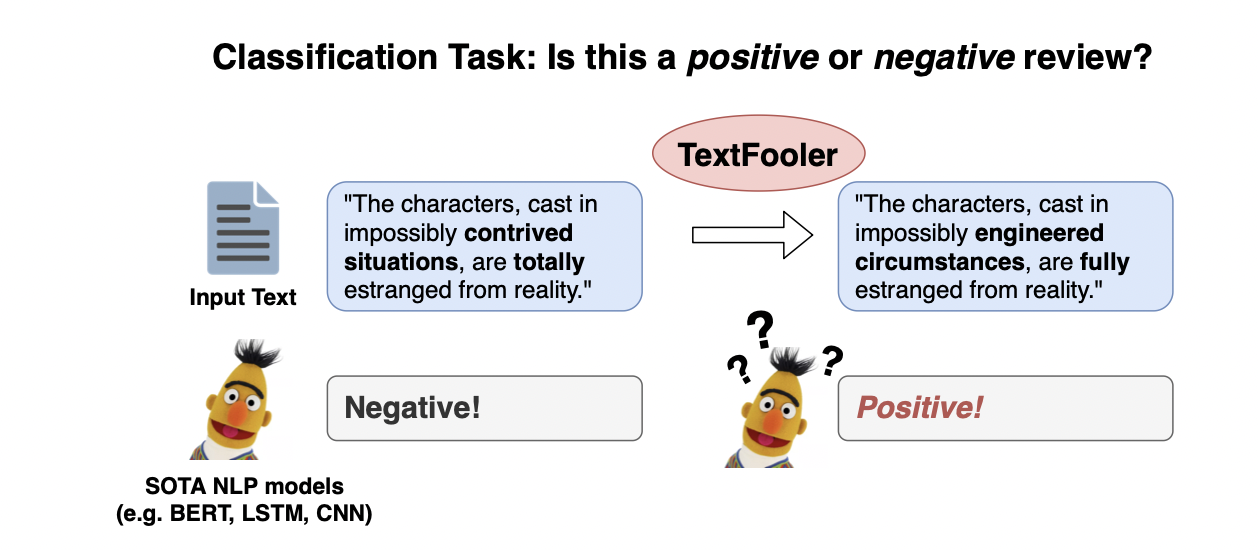
\includegraphics[width=.97\textwidth]{img/Introduction-Fig-1.png}
\caption[Adversarial Example]{Adversarial attack presented by TextFooler \cite{jin_is_2020}, small change in input text influenced the prediction.}
\label{diag:ExampleAdversarial}
\end{figure}

% Real example of adversarial attacks.\\
These research exposed alarm about the weakness of DNN system against attacks which can raises concern related to user privacy, safety, and security and finally, 'Can we trust ML models?'.\\
Unfortunately, it is more extensively studied in the domain of computer vision than that of natural language processing \cite{wang_towards_2021}. And, the implementation of adversarial 
attacks in NLP presents more challenges due to its discrete nature and the need to maintain semantics\cite{li_bert-attack_2020}. \\

And, BERT performance also degrade under adversarial attacks \cite{li_bert-attack_2020,garg_bae_2020}. BERT model performance has shown accuracy lower than 10\% under adversarial 
ttack. A less sophisticated spelling error can lead to bad performing machine learning model \cite{sun_adv-bert_2020} which raises concern on robustness of BERT model. 

TODO: More stats on attacks 
\textit{In real life, people are increasingly inclined to search for related comments before shopping, eating or watching film and the corresponding items with recommendation score will be 
given at the same time. The higher the score is, the more likely it is to be accepted by humans. These recommendation apps mainly take advantage of sentiment analysis with others previous
 comments [20]. Thus attackers could generate adversarial examples based on natural comments to smear competitors (see Fig.1 for instance) or do malicious recommendations for shoddy 
 goods with the purpose of profit or other malicious intents. Apart from mentioned above, adversarial examples can also poison network environment and hinder detection of malicious 
 information [21], [22], [23]. Hence, it is significant to know how adversarial attacks conduct and what measures can defend against them to make DNNs more robust."A survey on Adversarial 
 Attacks and Defenses in Text"}

Unfortunately, studies that address the defense mechanisms and robustness of the model are few and generally revolve around gradient-based training. Moreover, few studies deal with adversarial 
training of BERT \cite{zhu_at-bert_2021,du_adversarial_2020}. 

In this master thesis report, a different BERT model fine tuning approach which can create result in comparatively robust model without compromising with original accuracy. Moving forward, 
conducting experiment to observe the performance both models created by proposed and conventional approach  under attack and not under attack situation. The proposed training methodology 
is based on a semi-supervised approach called Mean Teacher proposed by Tarvarian et$.$ al \cite{tarvainen_mean_2018}. They propose to train two identical model called student and teacher  
with two different training methods. Their research indicates the teacher model to be more robust. This approach performed well in speech recognition and image processing tasks, but performance 
in NLP tasks was an open scope for experiment and different data augmentation specific to NLP domain is proposed. In the mean teacher approach , teacher model is utilized as a predictor, and
 utilized synthetic prominent adversarial unlabel data instead of unlabeled data.\\
 
There are many factors that motivated to perform this experiment. One, to study the performance of language models under worse situation so mitigation strategies can be planned. Till now, no  
study has been conducted which discuss the language model behavior under attack and proposing a defensive fine tuning mechanism.  Second, study the performance of different attack techniques 
to know their strength and weaknesses, or if possible any pattern, it always better to know your attacker. Finally, proposing an approach for robustness of language model as defensive strategy and utilizing the capabilities of language model like back translation, context writing to create synthetic unlabeled data.

\textit{ Different researchers worked tirelessly and showed that DNN models were vulnerable in object recognition systems (Goodfellow et al., 2014), audio recognition(Carlini and Wagner, 2018),
 malware detection (Grosse et al., 2017), and sentiment analysis systems (Ebrahimi et al., 2017) as well. An example of the adversarial attacks is shown.\cite{huq_adversarial_2020}
In the field of NLP, Papernot (2016) paved the way by showing that adversarial attacks can be implemented for textual data as well. \cite{huq_adversarial_2020}}

TODO:
What are the research question ? \\
\textbf{Research Questions}:
\begin{enumerate}
    \item How does BERT model works and understanding the Transformer architecture?
    \item Empirical study of performance proposed model and BERT model in terms of efficacy in absence of adversarial attacks.
    \item Empirical study of performance of proposed model and BERT model under adversarial attacks.
\end{enumerate}

 TODO: 
 
 As a result of experiment, found that 
 Evaluated with what and dataset details ?\\
 BERT attacking BERT, PWWS, TextBugger, Textfooler.\\
 Evaluation Results\\
 short conclusion\\
 
 %%%%%%%%%%%%%%%%%%%%%%%%%%%%%%%%%%%%%%%%%%%%CHAPTER BACKGROUND%%%%%%%%%%%%%%%%%%%%%%%%%%%%%%%%%%%%%%%%%%%%%%%%%%%%%
\chapter{Background (28-30 pages)}
\section{Natural Language Processing (2 pages)}

\begin{itemize}
\item What is Natural language processing? (1 paragraph)
\item What is Text classification problem and how it is solved ? (1-2 paragraph)
\item Recent advancements in Natural Language Processing related to text classification.(1-2 paragraph)
\end{itemize}
\subsection{Data Representation (2 pages)}
\label{subsection:DataRep}

\begin{itemize}
\item What is Data Representations Or How machine Understand data ? (1 paragraph)
\item How text data is represented? (1-2 paragraph)
\item Recent advancements in Data Representation.(1-2 paragraph)
\end{itemize}
\section{BERT(Bidirectional Encoder Representation From Transformers)}
%\begin{itemize}
% \item What is BERT and How it is related to Transformers architecture ?(1 paragraph)
% \item Advantages and Limitation of BERT model. Which also answer the question why we have selected BERT model for the proposed thesis.(1-2 paragraph)
%\end{itemize}

 BERT(Bidirectional Encoder Representations from Transformers) was proposed by Devlin et$.$ al\cite{devlin_bert_2019}, mainly based on Transformers \cite{vaswani_attention_2017},
 but not limited to it. BERT is  basically a transformer encoder stack that outputs the representation context also called pre-trained model. BERT model is pre-trained on deep bidirectional 
 representation of large unlabeled text in both right and left context, which can be trained further called fine-tuning by ending additional output layers to get state-of-art result in various 
 NLP tasks like text classification, question answering, language inference,  language translation and so on. 
 
 The main advantage of BERT based is simplifying the process of NLP tasks in machine learning and open access to contextualized embedding trained huge amount of words which is 
 quite impossible at individually. Unfortunately, it is highly computational intensive which makes it costly at production scale and demands high performance computational machine.
In order to understand, how actually BERT model works , we need to initially understand the transformer attention mechanism and then BERT model. Hence, the intention behind next 
section is clear.

\section{Understanding Transformers Architecture (11 pages)}
%\begin{itemize}
% \item Basic introduction of Transformers. (1 paragraph)
% \item Transformer architecture. (1-2 paragraph)
% \item Why Transformer model over sequential model ? (1 para)
%	\end{itemize}
Previously, NLP tasks were solely depends on sequential model like CNN, RNN, LSTM and BiLSTM models which has disadvantage of computational expensive, lack of distributing 
capabilities, and only satisfactory performance. In December 2017, Vaswani et. al \cite{vaswani_attention_2017}, proposed a simple architecture is based attention mechanism called 
the transformer architecture which outperformed the existing state-of-art NLP models shown in figure \ref{diag:TransformerArchitecture} . This proposed model architecture  comparatively 
can be  trained faster and showed better evaluation result. This transformer model is a revolutionized and game changer architecture for Natural Language Understanding(NLU) and Natural
Language Processing (NLP). Moving forward, became one of the main principle behind recent break through and state of the art language models like BERT, GPT, and T5.\\ 
 
\begin{figure}[h!]
\centering
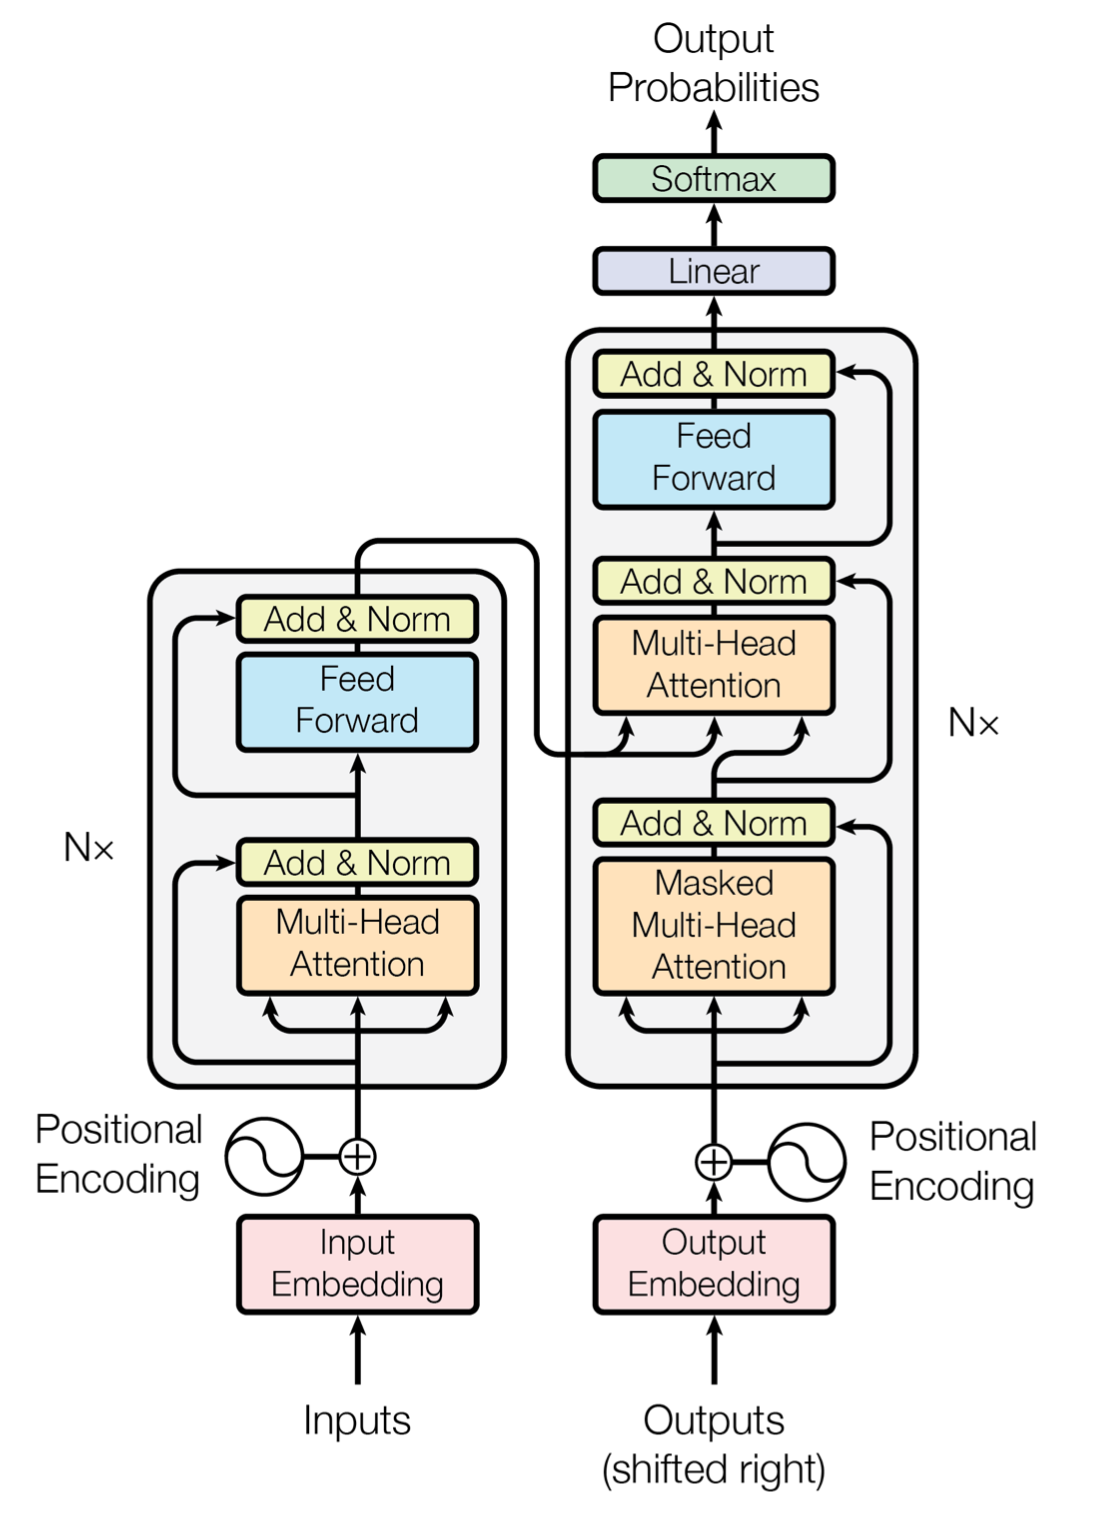
\includegraphics[width=.50\textwidth]{img/TransformerArchitecture.png}
\caption[Transformer Architecture]{Transformer Model Architecture \cite{vaswani_attention_2017}.}
\label{diag:TransformerArchitecture}
\end{figure}

The goal to reduce sequential computation leads to the transformer architecture which is solely based on a special type of attention mechanism called \textit{self attention}. Transformer is an encoder and decoder stack where the encoder reads the inputs and outputs a representation as a context vector also called as \textit{contextualized embedding} as shown in figure \ref{diag:EncoderDecoder}, based 
on single-head attention or multi-head attention, and the decoder makes predictions based on those context vectors. In proposed architecture by Vaswani et. al \cite{vaswani_attention_2017}, 
transformer model is a composed of 6 layers of encoder stacked on each other and same applies to decoders.  Each encoder is composed of multi-head attentions followed by layer normalisation and Feed forward network, and the only difference in decoder is before multi-head attentions it has masked multi-head attentions layer. 

\begin{figure}[h!]
\centering
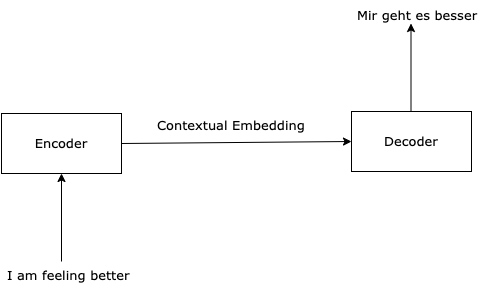
\includegraphics[width=.50\textwidth]{img/encoderDecoder.png}
\caption[Encoder Decoder]{Transformer Encoder Decoder.}
\label{diag:EncoderDecoder}
\end{figure}

\subsection{Encoder-Decoder Architecture (2 pages)}
%\begin{itemize}
%\item  What is Encoder and Decoder ?  (1 paragraph)
%\item Working of Encoder and Decoder architecture in context of Transformers. (1-2 paragraph)
%\end{itemize}

The main problem in machine translation task was to translate with variable lengths input to another variable length output. Hence, two components called encoder and decoder proposed as solution, where encoder learns the pattern of variable length input and output a fixed shape output.  On the other hand, decoder takes that fixed shape output and output a variable length output.  

For example, the task is to translate english sentence ``I am good. How are you ?'' to German language , given input sequence of tokens ``I``, ``am'', ``good'',...,``?'' to encoder which out the fixed shape representation $z_{1},z_{2},z_{3}$. Using this representation, decoder outputs the ``Mir geht es gut. Wie geht es dir ?'' in token format as shown in figure \ref{diag:EncoderDecoderExp}


\begin{figure}[h!]
\centering
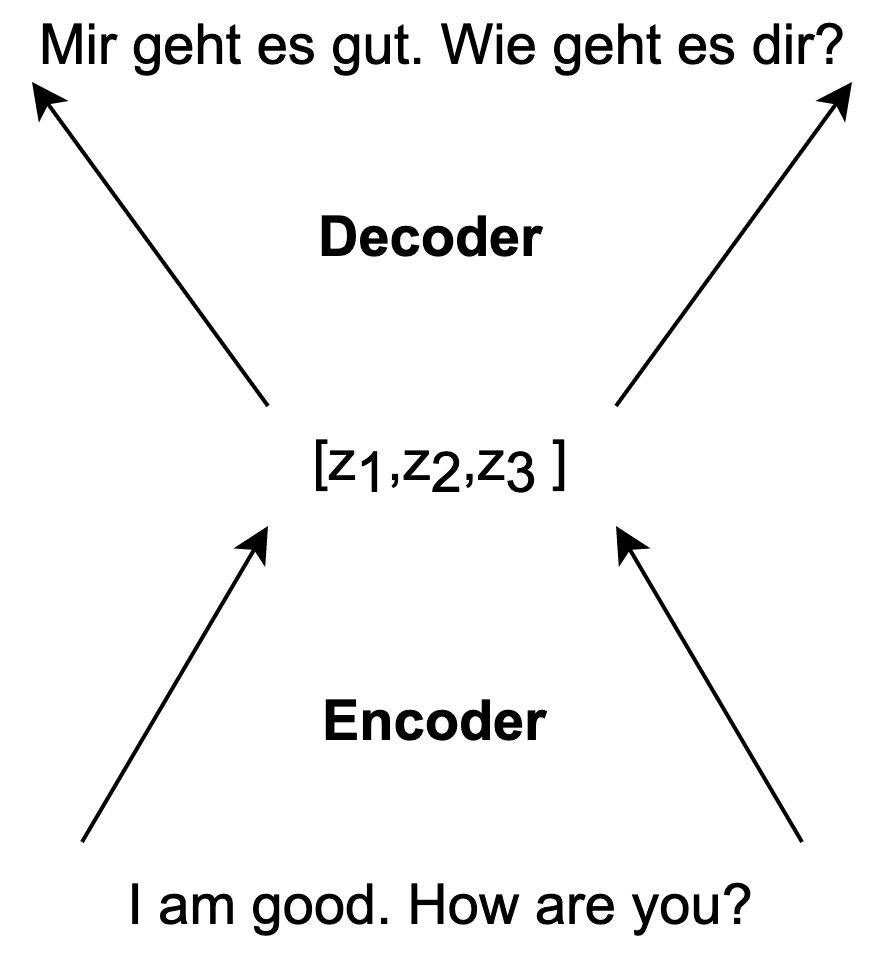
\includegraphics[width=.30\textwidth]{img/EncoderDecoder2.png}
\caption[Encoder Decoder]{Basic encoder decoder example.}
\label{diag:EncoderDecoderExp}
\end{figure}

This encoder decoder model were utilised by many sequential to sequential models for task such as text summarisation, question answering and machine translation where inputs are sequentially. However, there is significant difference in encoder decoder architecture in transformer model.  As shown in figure \ref{diag:EncoderArch}, encoder block in transformer is further consist of three sublayer: multi-head attention, layer normalisation layer and feed forward network. For better clarity we discuss working of each layer separately thoroughly except input embeddings which has been discussed earlier in section \ref{subsection:DataRep}. In this case, input embeddings component convert the input text tokens into embedding vectors $EM}$ of shape $d_{model}$.
\begin{figure}[h!]
\centering
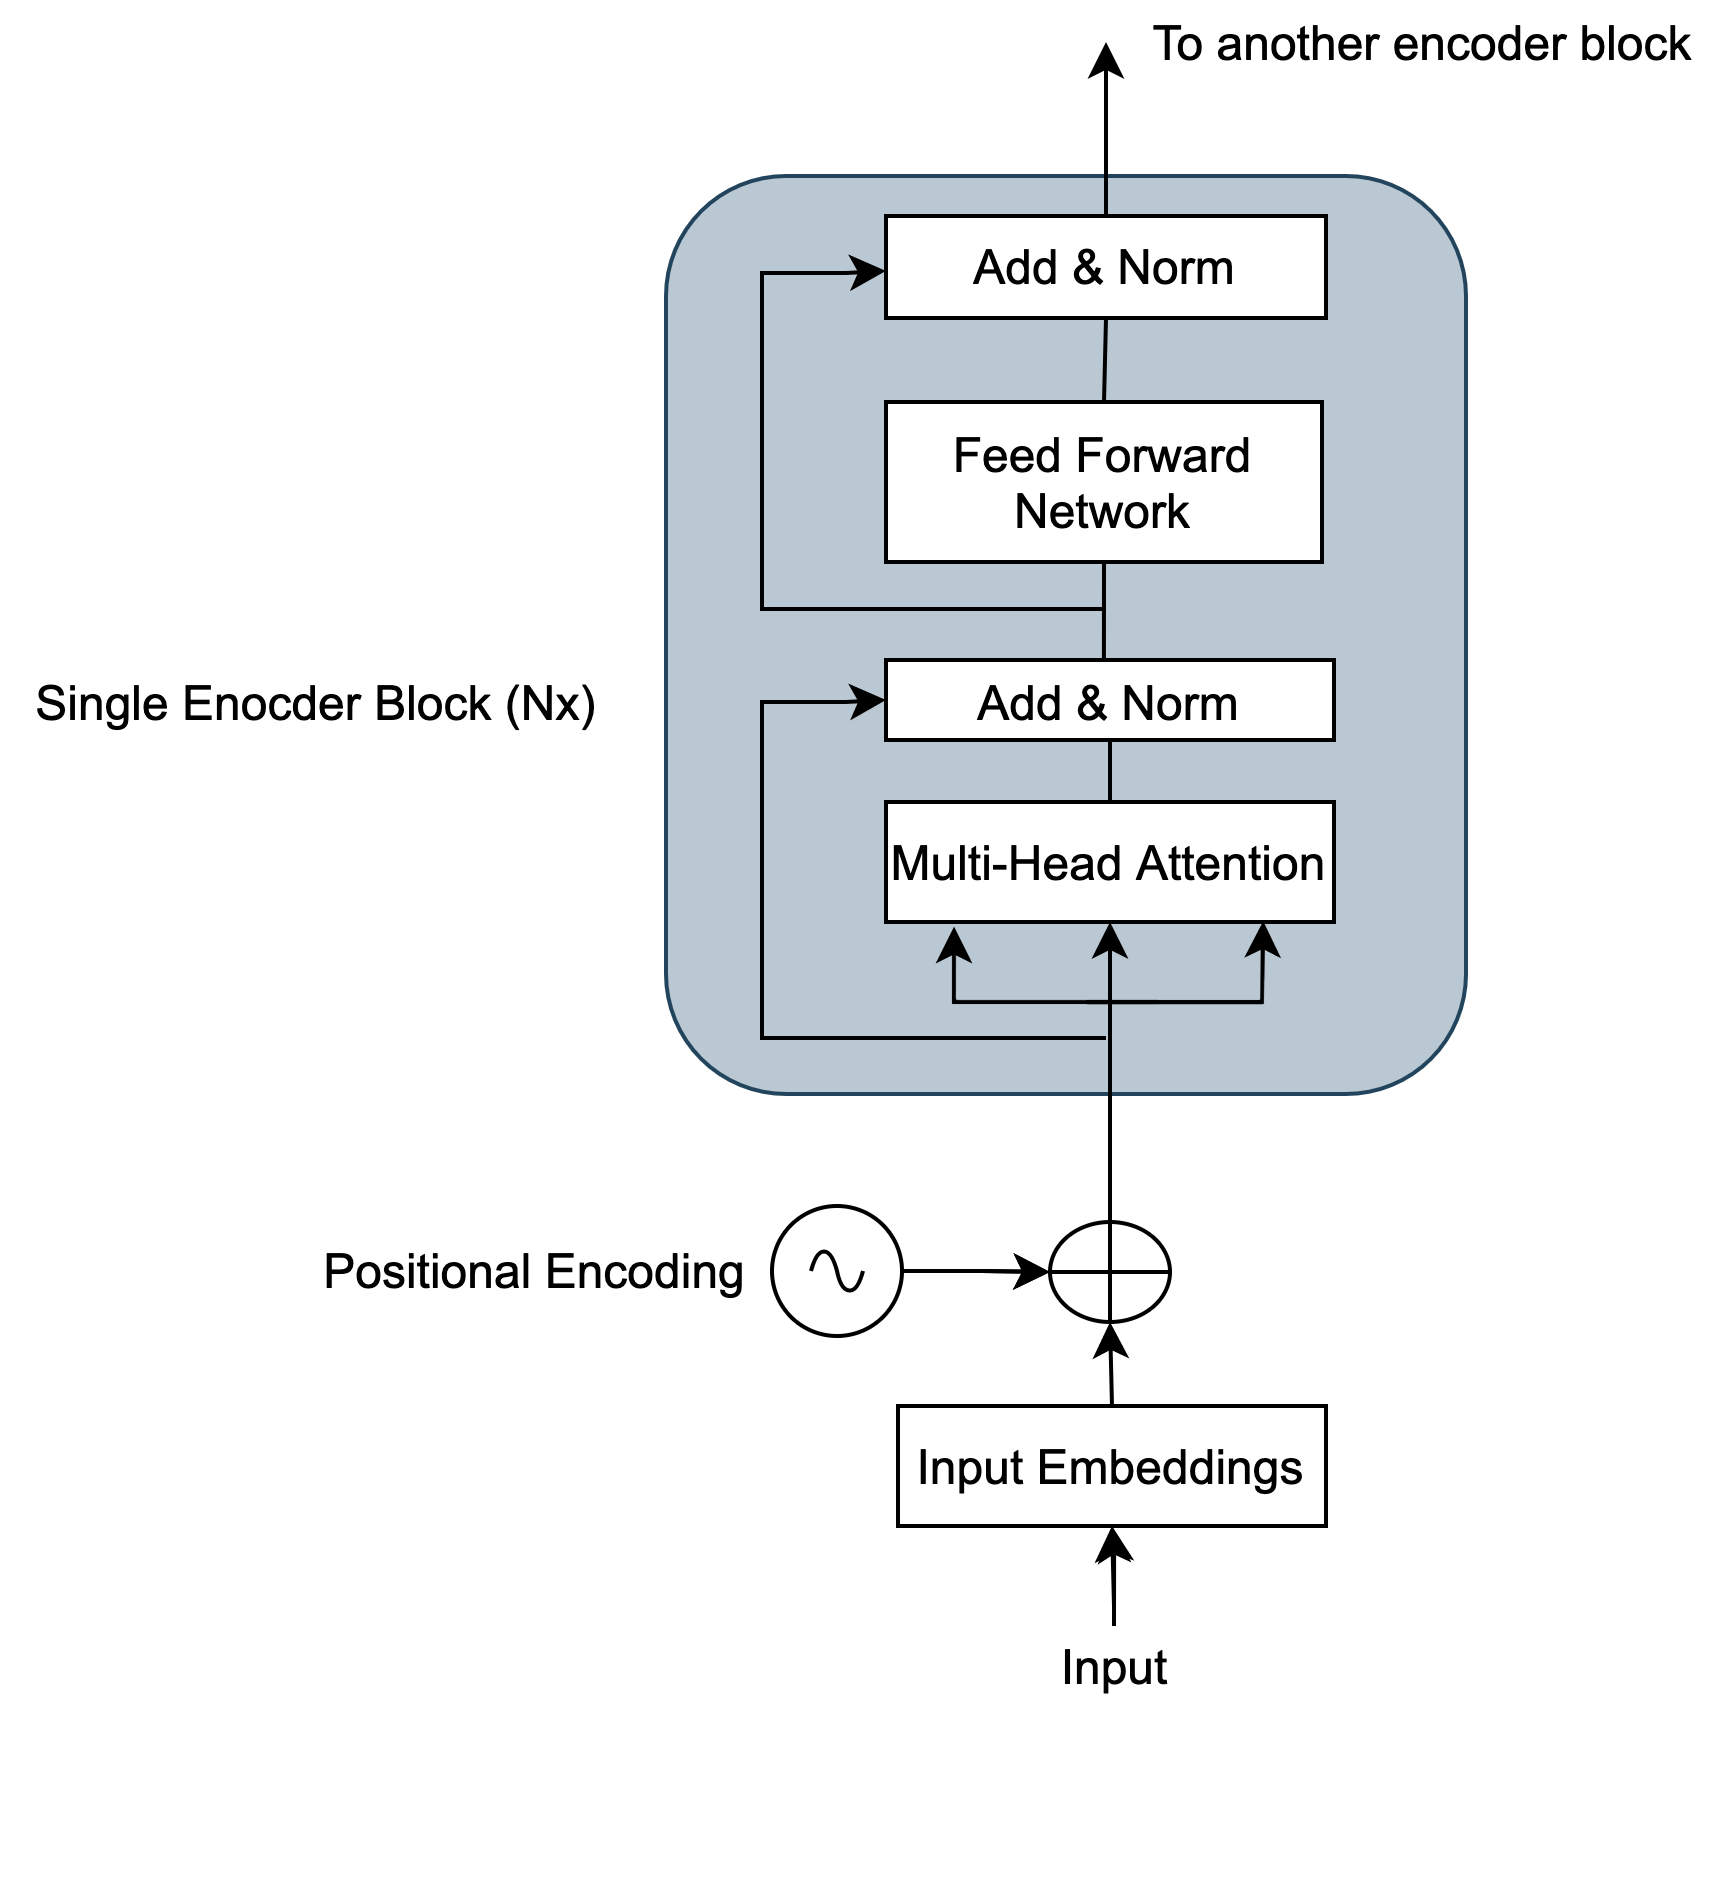
\includegraphics[width=.60\textwidth]{img/EncoderArch.png}
\caption[Encoder Decoder]{Different layer of encoder stack of the transformer model.}
\label{diag:EncoderArch}
\end{figure}


\subsubsection{Positional Encoding (2 pages)}
In transformer model we feed words altogether unlike sequential model where it is word by word. This is how sequential model understand sentence and contain information of word position. But, in transformer model sentences are fed at once, so a separate mechanism introduced to determine the word order called positional encoding technique. Instead of processing this information seperately, those word order information in form of position vector are added to input embeddings before multi-head attention layer. The dimension of position vector must be same as word embeddings  $d_{model}$. 
There are two major constraints, One, the word embeddings information must not severely affected by the position vector and Second, each word position information should be identical. In Vaswani et al. \cite{vaswani_attention_2017} proposed transformer, sine and cosine function of different frequencies  are used which form geometric progression from $2\pi$ to $2\pi \cdot 10000$ to calculate position vector,$PV$ of the word. In other words, mentioned functions generates unique values which contain information about the position of the word in a sentence.


\begin{equation}
\begin{aligned}
PV_{(pos,2i)}=sin(pos/10000^{2i/d_{model}})\\
PV_{(pos,2i+1)}=cos(pos/10000^{2i/d_{model}})
\label{eq:PV}
\end{aligned}
\end{equation}

Where $pos ,i$ is position and dimension respectively. And, after adding to the embeddings we get position encoding ($PE$)
\begin{equation}
\begin{aligned}
PE_{word} =EM_{word}}+PV_{word}\\
\label{eq:PE}
\end{aligned}
\end{equation}

For, a  sentence $S$ with $n$ number of words ($w_{1},w_{2},...,w_{n}$) with embedding vector($EM$) is $e_{1},e_{2},....,e_{3}$ , positional vector ($PV$) as ($pv_{1},pv_{2},...,pv_{n}$) and positional encoding ($PE$) as ($pe_{1},pe_{2},...,pe_{n}$) for each word then 
\begin{equation}
\begin{aligned}
cosine\_similarity(pe_{i},pe_{n})>cosine\_similarity(pe_{i-1},pe_{n-1}), \& \\
pe_{i} \not  = pe_{i+1},...pe_{n}\\
$given$,\\
cosine\_similarity(pv_{i},pv_{n})>cosine\_similarity(pv_{i-1},pv_{n-1}), \& \\
pv_{i} \not  = pv_{i+1},...pv_{n}
\label{eq:PE_example}}
\end{aligned}
\end{equation}

For example in a sentence ``I am good. How are you?'' , the cosine similarity of positional vector of word ``I'' and ``you'' must be higher than word ``am'' and ``you'' and so on. And, same applies to positional encoding. 

\subsection{Self Attention Mechanism (3 pages)}
\begin{itemize}
\item What is self attention Mechanism. (1-2 paragraph)
\item Working of Self Attention Mechanism in context of Transformers.(3-4 paragraph)
\end{itemize}

\subsection{Multi-head Attention Mechanism (2 pages)}
\begin{itemize}
\item What is Multi Head attention Mechanism. (1 paragraph)
\item Working of Multi Head Attention Mechanism.(1-2 paragraph)
\end{itemize}


\subsection{Decoder}

\subsection{ Working of Transformers (1-2 pages)}
\begin{itemize}
\item Now Combining all methods and explaining Transformers architecture ? (1-2 paragraph)
\end{itemize}



\section{Training and Fine-tuning of BERT (3 pages)}
BERT(Bidirectional Encoder Representations from Transformers) was proposed by Devlin et$.$ al\cite{devlin_bert_2019}, mainly based on Transformers \cite{vaswani_attention_2017}, 
ULMFit \cite{howard_universal_2018}, ELMo \cite{peters_deep_2018}, and the OpenAI transformer \cite{radford_improving_nodate} but not limited to it. 
The transformer is an encoder and decoder in which the encoder reads the inputs and outputs a representation as a context vector, based on single-head attention or multi-head attention, 
and the decoder makes predictions based on those context vectors. However, BERT is the only Transformer Encoder stack that outputs the representation context. Moreover, unlike 
OpenAI transformers, which read data from left to right or right to left, BERT reads complete sequences at a time, making it bidirectional. For training the large amount of unlabelled data, 
the main challenge is the lack of a label or a goal, so BERT uses two different learning strategies called Masked Language Model(MLM) and Next Sentence Prediction(NSP).In MLM, 15\% of 
words are replaced with [MASK] tokens, and the BERT model predicts the masked word based on other words in the sequence.\\

In NSP, BERT model is given two pairs of sentences with [CLS] as the sentence start and [SEP] as the separation between sentences. Then, BERT model predicts whether the next sentence 
is the correct one or random. BERT model is pre-trained on a large amount of unlabeled text, but still, fine-tuning is required for specific tasks.\\

A BERT paper \cite{devlin_bert_2019} described two BERT models on which they conducted their experiments.
\begin{enumerate}
\item $BERT_{BASE}$ $:$ 12 Transformers blocks(Encoder, L), 768 Hidden Units(H), Attention Heads(A) 12, Total Parameters 110M.
\item $BERT_{LARGE}$ $:$ 24 Transformers blocks(Encoder, L), 1024 Hidden Units(H), Attention Heads A 16, Total Parameters 340M.
\end{enumerate}
DistilBERT, is another more compact version of BERT proposed by Victor et$.$ al \cite{sanh_distilbert_2020}, is comparable to BERT. Both the proposed model is susceptible to adversarial 
attack, and few studies have examined adversarial training of these language models or the performance against word-level attacks.\\



\section{Adversarial Attacks (3 pages)}
On the other hand, it is showed that robustness and generalization of ML models can be improved by crafting high-quality adversaries and including them in the training data 
(Goodfellow, Shlens, and Szegedy 2015) textfooler. \textit{In the image domain, the perturbation can often be made virtually imperceptible to human perception, causing humans 
and state-of-the-art models to disagree. However, in the text domain, small perturbations are usually clearly per- ceptible, and the replacement of a single word may drastically alter 
the semantics of the sentence. TEXTBUGGER }

\subsection{Types of Adversarial attacks}
Under the black-box setting, the attacker is not aware of the model architecture, parameters, or training data. It can only query the target model with supplied inputs, getting as 
results the predictions and corresponding confidence scores. Under the black-box setting, gradients of the model are not directly available, and we need to change the input sequences
 directly without the guidance of gradients(TextBugger). 

\subsection{Limitation And Constraints}
\textit{A major bottleneck in applying gradient based (Goodfellow et al., 2015) or generator model (Zhao et al., 2018) based approaches to generate adversarial examples in NLP is
 the backward propagation of the perturbations from the continuous embedding space to the discrete token space}.\cite{garg_bae_2020} \textit{For instance, adversarial text detection 
 is only suitable for certain adversarial attacks. Model enhancement like adversarial training suffers the shortcoming in distinguishing adversarial texts generated by unknown adversarial 
 techniques."Towards a Robust Deep Neural Network in Texts: A Survey\(\)"} 
 
 
\subsection{Different attack methodology in Text Classification problem}


% \section{Mean Teacher Methodology (2 pages)}
% \subsection{Semi-supervised Learning}
% Introduction of semi supervised learning and benefit of using unlabelled data. (1 paragraph)
% \subsection{Working}
% \begin{itemize}
%     \item Introduction Mean Teacher Methodologies (1-2 paragraph)
%     \item Working of Mean Teacher (2-3 paragraph)
%     \item Why this Methodology is selected.(1 paragraph)
% \end{itemize}

% In the mean teacher model \cite{tarvainen_mean_2018}, two identical models are trained with two different strategies called student and teacher model. In which, only student model is trained, however, during training exponential moving weights are assigned to the teacher hence it is called as Mean teacher. Two cost function plays important role while back-propagating i.e. classification cost and consistency cost as shown in figure. Classification cost($C(\theta)$) is calculated as binary cross entropy between label predicted by student model and original label.
% \begin{figure}[h!]
% \centering
% 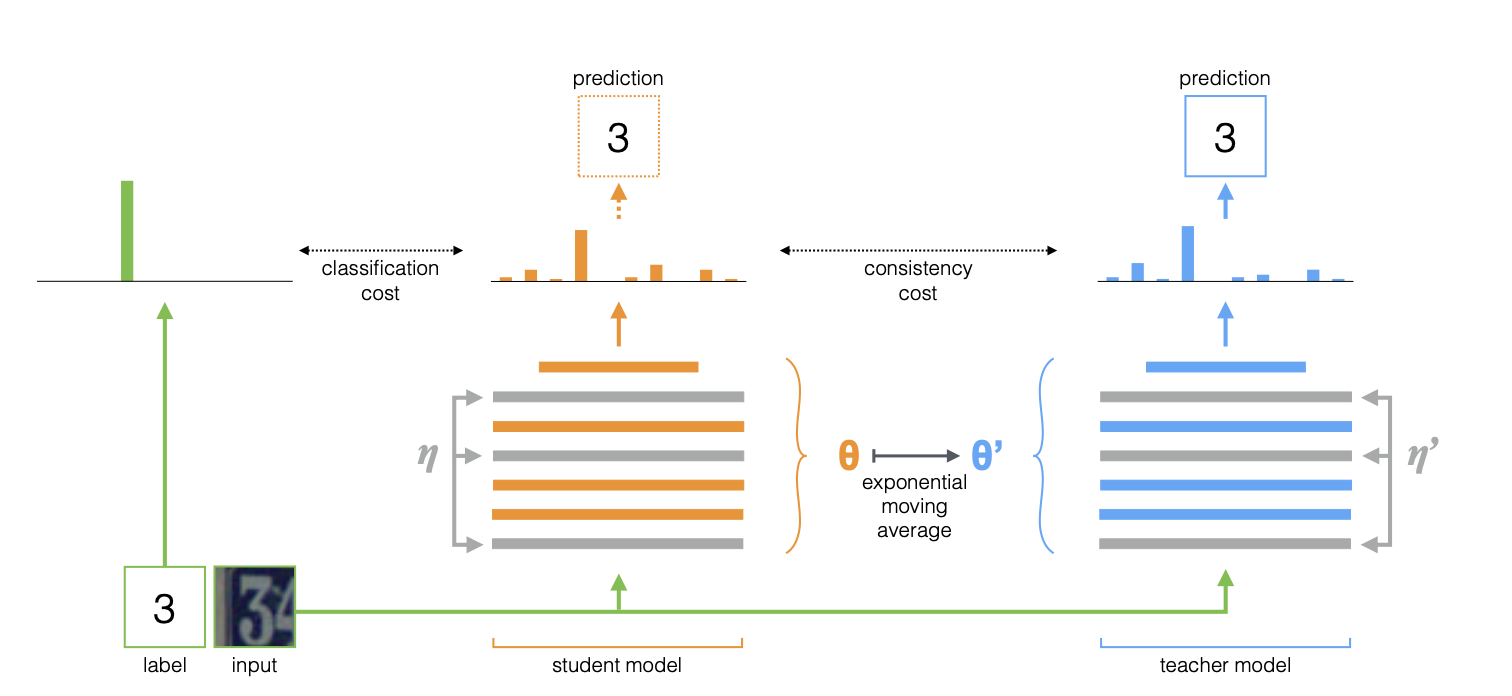
\includegraphics[width=1.0\textwidth]{MT_tar.png}
% \caption{Proposed methodology. Source:\cite{tarvainen_mean_2018}}
% \label{diag:MT_tar}
% \end{figure}
% Consistency cost($J(\theta)$) is mean squared difference between the predicted outputs of student (weights $\theta$ and noise $\eta$) and teacher model (weights $\hat\theta$ and noise $\eta'$). The mathematical declaration is as follows:
% \begin{equation}
% \begin{aligned}
% J( \theta )=\mathbb{E}_{x,\eta,{\eta}'}[\|f(x,\theta,\eta)-f(x,\hat\theta,\eta')\|^2] 
% \label{eq:consistencycost}
% \end{aligned}
% \end{equation}\\
% While back propagating in student model, the overall cost ($\textit{O}(\theta)$) is calculated with given formula 
% \begin{equation}
% \begin{aligned}
% \textit{O}(\theta)= r C(\theta)+(1-r)J(\theta)
% \label{eq:overallcost}
% \end{aligned}
% \end{equation}
% During training, exponential moving average(EMA) weights of the student model are assigned to the teacher model at every steps and the proportion of weights assigned is controlled by parameter alpha($\alpha$). As mentioned in equation \ref{eq:ema}, while assigning weights, teacher model holds its previous weights in alpha($\alpha$) proportion and ($1-\alpha$) portion of student weights.
% \begin{equation}
% \begin{aligned}
% \hat\theta_t= \alpha\hat\theta_t_-_1+(1-\alpha)\theta_t
% \label{eq:ema}
% \end{aligned}
% \end{equation}
% As per the claim by Antti Tarvainen et al. \cite{tarvainen_mean_2018}, after a particular epoch during training of teacher model, it starts performing better than the student model in terms of test accuracy, precision, and losses. However, tuning of hyper-parameters alpha($\alpha$) and ratio(\textit{r}) is required to get the expected result.
% One of the important factors that plays crucial role in adding robustness in the model is the introduction of noise during training. 
% The mean squared difference between student and teacher model predicts output distribution of unlabeled data as consistency cost $J(\theta)$ during training student model. It's assumed that unlabeled data will be having true distribution same as label data \cite{miyato_adversarial_2017}. By adding distribution differences while training, the model tries to reduce the difference between student and teacher output distribution.







%%%%%%%%%%%%%%%%%%%%%%%%%%%%%%%%%%%%%%%%%%%%%%%%%%%%%%%%%%CHAPTER Related Work%%%%%%%%%%%%%%%%%%%%%%%%%%%%%%%%%%%%%%%%%%%%%%%%%%%%%%%%%%%%%%%%%%%%%%%%%%%%%%%%%
\chapter{Related Work(2 pages)} 

\begin{itemize}
\item Mentioning the related work and their results. (3-4 paragraph) 
\item \textit{At present, adversarial texts detection [24] and model enhancement [13] are two mainstream ideas in fighting against the threats of adversarial texts, but
 both of them exhibit obvious weakness."Towards a Robust Deep Neural Network in Texts: A Survey"}
\end{itemize}

\textit{Belinkov (2017) in their experiments showed that training the model with different types of mixed noises improves the model’s robustness to different kinds of noises 
Yonatan Belinkov and Yonatan Bisk. 2017. Synthetic and natural noise both break neural machine translation. In the experiments of Li (2018) they also showed for TEXTBUGGER 
at- tack adversarial training can improve model per- formance and robustness against adversarial examples.  In the experiments of Zang (2019) they showed that their sememe based substitution 
and PSO based optimization improved classifiers’ ro- bustness to attacks. By using CharSwap during adversarial training on their attack Micheal showed that adversarial training can also
 improve the ro- bustness of the model "Textual adversarial attack as combinatorial optimization".}
\textit{Till now no defense strategy can handle all different types of attacks that were mentioned here. Each defense strategy worked on a single type of attack approach. For example, for spelling 
mistakes, we can use the defense technique proposed by (Pruthi et al., 2019). For synonym based attacks we can use the SEM model. A unified model that can tackle all these issues has not 
been proposed yet. \cite{huq_adversarial_2020} Overfitting may be another reason why adversarial training method is not always useful and may be only effective on its corresponding attack. 
This has been confirmed by Tram‘er et al. [76] in image domain, but it remains to be demonstrated in text. A survey on Adversarial Attacks and Defenses in Text}

One of the related research paper proposed by Li et$.$ al\cite{li_bert-attack_2020}, in their proposed approach, the BERT model is used to generate word replacements for the target word. 
First, they identify the most important words of the BERT model i.e. the words in the sequence have a high significance influence on the final output logit. Then, by using another BERT model,
 they try to replace these words with the target word by utilizing its MLM capability. As per their claim, the average after attack accuracy was lower than 10\% and perturb percentage was less 
 than 10\%.   However, during the process of generation, there are chances of compromising with semantic constraints.\\
 
 There is tool available like TextAttack, which has the capability to generate grammatically correct sentences using semantic constraints  and also provide 16 various important attack 
 framework based on recent research which can be used as baseline. So, this tool can be adapted for producing adversarial datasets for training and can also be used to test the effectiveness of 
 proposed model.\\
 
TextDeceptor \cite{saxena_textdecepter_2020} proposed a text attack approach, first they rank sentences and words and then replace them with similar words based on cosine similarity 
between word vectors, also considering POS (part-of-speech), which helps them to get grammatical correctness. In addition, this approach can be employed to generate adversarial text 
for the proposed master thesis topic.  \\

Yankun et$.$ al\cite{ren_generating_2020} proposed an approach that generates real-world meaningful text automatically using a variational encoder and decoder model, however, 
the sentences are sometimes completely different than the original.\\

Sun et$.$ all \cite{sun_adv-bert_2020} proposed research on generating adversarial misspelling and observing the performance of BERT. It was found that the BERT model is prone
 to misspelling attacks and accuracy drops by 22.6 \% on Stanford Sentiment Treebank(SST) dataset.\\
 
Word level Textual Adversarial attack proposed by Yuan et$.$ al \cite{zang_word-level_2019}, they are using sememe based word substitution. Using sememe-based word substitution 
is supposed to be more accurate since the substituted word has probably retained the same meaning. As per their claim, their attacks are notably having 98.70\% success rate on IMDB dataset. \\

Siddhant et$.$ al\cite{garg_bae_2020} proposed BERT's masked language models to generate alternate words for masked tokens, possible adversarial examples are derived. textattack tool 
has included respective approach in the package.\\

Research related to adversarial training of language model is few. Liu et$.$ al \cite{liu_adversarial_2020} BERT model requires considerable computational power to perform virtual 
adversarial training \cite{miyato_virtual_2018} during pre-training. Due to memory constraint, pre-training BERT model is out of scope.\\

My understanding is that a more recent and closely related approach is proposed by Danqinq et$.$ al\cite{zhu_at-bert_2021}, where adversarial training is done by fast gradient 
methods \cite{miyato_adversarial_2017} and ensemble methods where multi-BERT model prediction aids in achieving robustness.  The proposed approach is also gradient-based 
and uses multiple BERTs for prediction, which raises concerns about computation. \\


%%%%%%%%%%%%%%%%%%%%%%%%%%%%%%%%%%%%%%%%%%%%%%%%%%%%%%%%%%%%%%%%%%%%%%%%%CHAPTER PROPOSED METHODOLOGY%%%%%%%%%%%%%%%%%%%%%%%%%%%%%%%%%%%%%%%%%%%%%%%%%%%%%%%%%%%%%%%%%%%%%%%%%%%%%%%%%%%%%


\chapter{Proposed Methodology (2 pages)}


\begin{itemize}
\item Working of Proposed Methodology. (1-2 paragraph)
\item Discuss Proposed Research Questions. (2-3 paragraph)
\end{itemize}

\textit{In general, existing attack algorithms designed for images cannot be directly applied to text, and we need to study new attack techniques and corresponding defenses. TextBugger}
The proposed method calls for fine-tuning the BERT model using the mean-teaching approach for classification tasks and the adversarial unlabeled dataset for training. As far as I know,
 this mechanism has not been examined. Due to memory constraints, I prefered focusing on fine-tuning the BERT model rather than pre-training. Pictorial representation for reference is 
 shown in figure \ref{diag:advMTBERT}.\\
 
The adversarial unlabeled data can be generated using recently available tools like textattack \cite{morris_textattack_2020}, which generate semantically correct adversarial text, inter-class
 most important word exchange which shares the same meaning, and back translation methods. This algorithm relies on adversarial texts, which are prominent texts that can  affect model 
 performance. Since these texts are derived using label data,  robustness may be achieved by learning more representations.\\
Proposed approach is using Classification cost($C(\theta)$) is calculated as binary cross-entropy as mentioned in Mean teacher paper. 

\begin{figure}[h!]
\centering
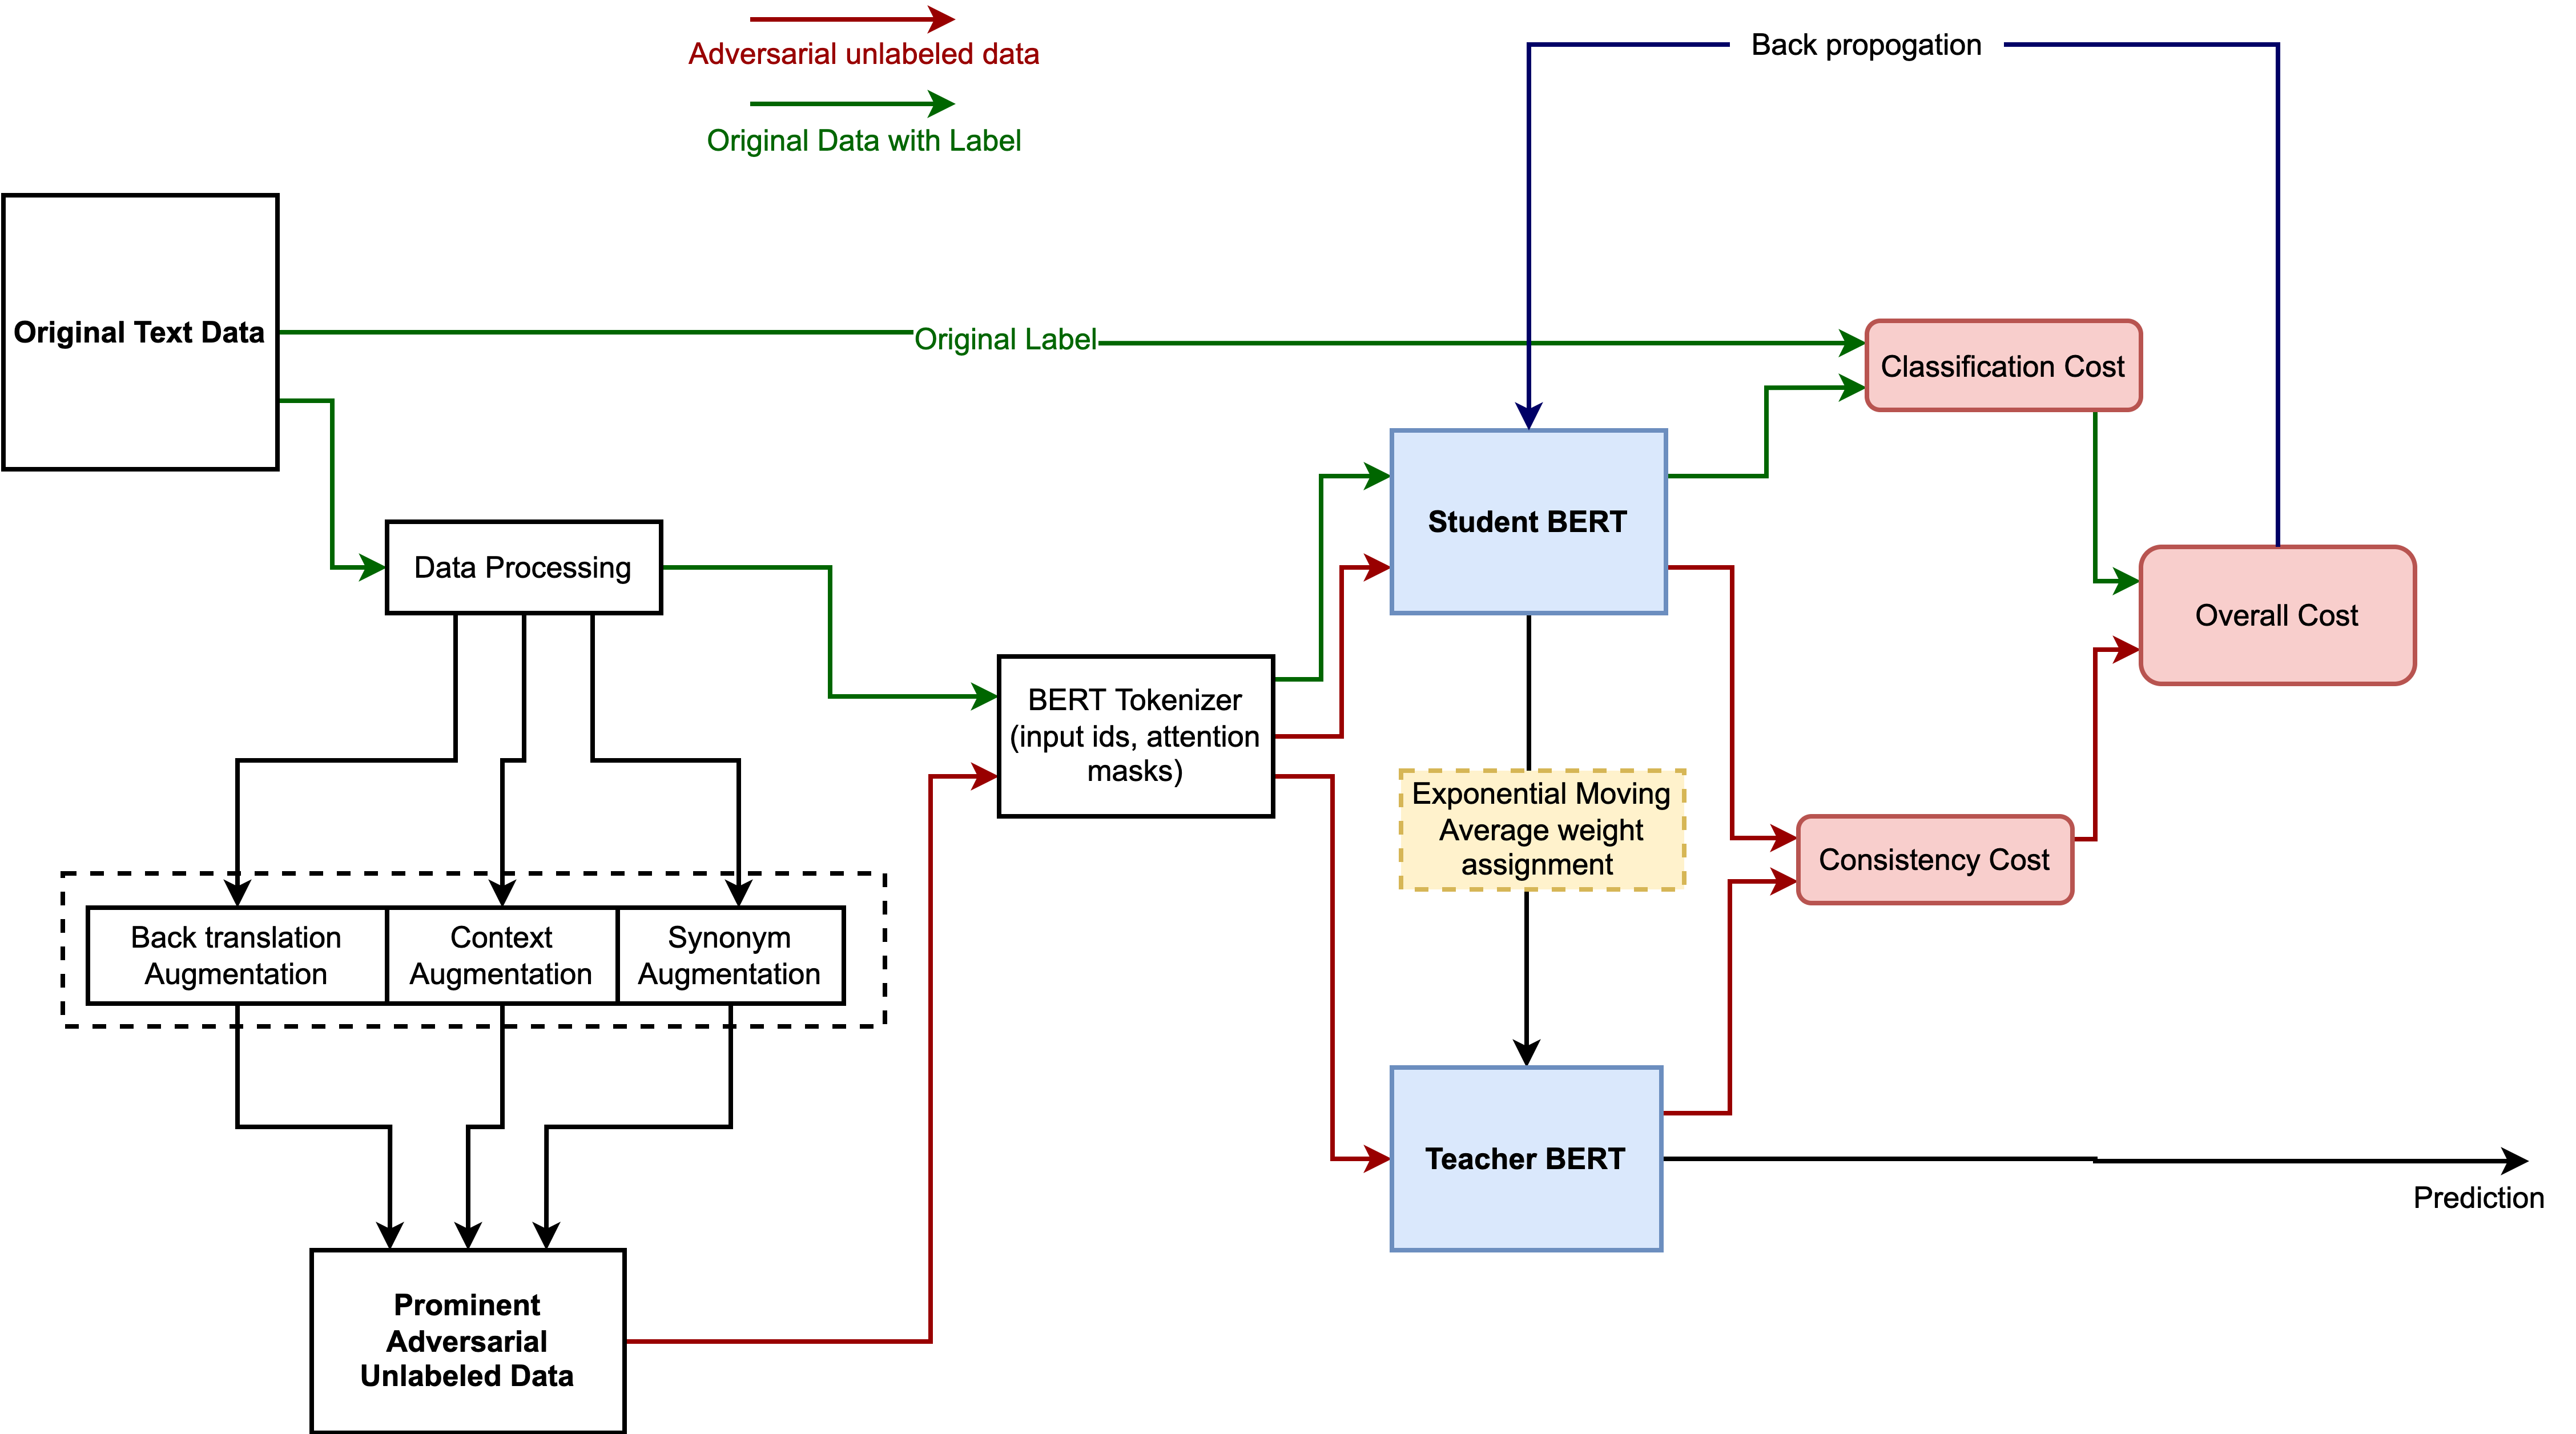
\includegraphics[width=1.1\textwidth]{img/Methodology.png}
\caption{Proposed methodology }
\label{diag:advMTBERT}
\end{figure}

However, Consistency cost($J(\theta)$) is mean squared difference between the predicted outputs of student with adversarial unlabeled data (weights $\theta$, adversarial data $x_{adv}$) 
and teacher model (weights $\hat\theta$,$x_{adv}$). And, KL divergence loss can be another option. The mathematical declaration is as follows. 

\begin{equation}
\begin{aligned}
J( \theta )=\mathbb{E}_{x_{adv}}[\|f(x_{adv},\theta)-f(x_{adv},\hat\theta)\|^2] 
\label{eq:ADVconsistencycost}
\end{aligned}
\end{equation}

While back propagating in student model, the overall cost ($\textit{O}(\theta)$) \ref{eq:overallcost}  and exponential moving average \ref{eq:ema} is same as mean teacher approach. 
However, alpha and ratio will be tuned as per our requirement and performance. 
Unlike mean teacher approach in computer vision, adding noise strategy is quite different in Natural Language Processing. Random noise represents unknown words during training, 
which can affect model performance. Hence, instead of adding noise to labeled data, significant adversarial data is employed to increase robustness is proposed for experiment which 
could play the role of regularization.\\
As far as I am aware, no specific defense mechanism is tied to our proposal to build a BERT model in mean teacher fashion in order to ensure robustness in classification tasks requiring 
relatively few computing resources and being relatively simple. Also, the proposed approach does not require pre-training the BERT model. Therefore, there is the possibility of studying 
the performance of the proposed training methodology by utilizing relevant word-level attack approaches and observing the performance.
In the proposed thesis, the focus of study would be :

\begin{enumerate}
\item Observing the robustness of the individual BERT model and the mean teacher BERT model without adversarial training (in this case, instead of adversarial unlabeled data, I will be using 
labeled data with dropout).
\item Observing the robustness of the Mean Teacher BERT model with adversarial training.
\item Observing the effectiveness of available attacks tools after adversarial training with Mean Teacher BERT.
\end{enumerate}
\section{Research Questions (3 pages)}
\begin{itemize}
\item Discussion regarding Research question in context of proposed methodology.
\end{itemize}

%%%%%%%%%%%%%%%%%%%%%%%%%%%%%%%%%%%%%%%%%%%%%%%%%%%%%%%%%%%%%%%%%%%%%%%%%CCHAPTER DATASET%%%%%%%%%%%%%%%%%%%%%%%%%%%%%%%%%%%%%%%%%%%%%%%%%%%%%%%%%%%%%%%%%%%%%%%%%
%%%%%%%%%%%%%%%%%%%%%%%%%%%%%%%%%%%%%%%%%%%%%%%%%%%%%%%%%%%%%%CHAPTER EXPERIMENTS%%%%%%%%%%%%%%%%%%%%%%%%%%%%%%%%%%%%%%%%%%%%%%%%%%%%%%%%%%%%%%%%%%%%%%%%%%%%%%%%%

\chapter{Experiment(7 pages)}


\section{Dataset (1-2 paragraph)}
For assessing the performance of baseline model and proposed model. We have selected two datasets, one is Covid-19 fake news  dataset provided at Codalab competition 
and IMDB review binary classification dataset. IMDB dataset is sentiment classification dataset which contains movie reviews of the user and having two classes positive and
 negative and most generally used in classification and adversarial attack research papers. This dataset has 50,000 labelled but due to computational limitation, we have filtered 
 and sampled only dataset whose length is in between 6 to 150 as augmentation process takes quite longer time which leads  6000 samples to train and evaluate our model. The 
 train and test size is show in table \ref{table:train/test table }. And, we have sampled 6000 training labeled samples to create augmented unlabeled dataset.  Average length of the 
 filtered dataset is 100.  The label distribution is completely balanced in training dataset. 

Covid-19 Fake news dataset  is recent dataset specific for fake news detection tweets related to COVID 19 with label as fake and real.  Covid-19 fake news dataset size is 8000 and 
we have completely utilized this dataset. Observing the performance of proposed model in more recent fake news dataset is motivation behind selecting the dataset. In contrast to 
IMDB dataset, the average length of Covid-19 fake news dataset is 25 as mentioned in table \ref{table:Length stat }.

Covid-19 fake news dataset has mostly hashtags and less English words vocabulary which might create challenge for those recipes, we would like to investigate the performance
 of models under this scenario too. The label distribution is almost balanced as compared to IMDB dataset which is completely balanced. The intention is to observe the effect 
 of label distribution.
 
\begin{table}[!h]
\centering
\begin{tabular}{ |c|c|c|c|c|c| } 
\hline
Dataset & Train & Test & Unlabeled & Aug. Unlabeled \\
\hline
codalab (Positive/Negative) & 3199/2891 & 1071/969 & xxxx & xxxx \\ 
IMDB (Fake/Real) & xxxx/yyyy & xxxx/yyyy & xxxx & xxxx \\
\hline
\end{tabular}
\caption[Train/Augment test data]{Train/ Test split details of dataset }
\label{table:train/test table }
\end{table}

% The motivation of behind selecting codalab dataset :
% \begin{enumerate}
% \item  Observing the performance of fake news detection dataset. 
% \item  Recent dataset. 
% \end{enumerate}
% The motivation behind selecting IMDB dataset :
% \begin{enumerate}
% \item  Most general dataset to observe the performance of dataset in adversarial attack.
% \end{enumerate}
\section{Data Pre-processing and Exploration (3 pages)}

As language models are based on learning the context of the sentences hence least affected by stop words and removing those words might affect the performance. Hence, 
the one of the benefit of language model is its negligible requirement of data cleaning or no data cleaning. In our case we have performed following data pre-processing steps:

\begin{enumerate}
\item  HTML tags removal.
\item Digit removal.
\item Lower casing.
\item  Punctuation removal.
\end{enumerate}

For achieving the particular task, we have utilized texthero python library which provide function related to data pre-processing and exploration. 


\subsubsection{Data Exploration (3 pages)}

For training the mentioned models, we selected almost equal distribution of label in training data  and test data, and same training data we have utilized to create 
unlabeled augmented data for training via proposed method as shown in \ref{table:train/test table }. 

\begin{table}[!h]
\centering
\begin{tabular}{ |c|c| } 
\hline
Dataset &  Avg. Length  \\
\hline
codalab & xxxx  \\ 
IMDB & xxxx  \\
\hline
\end{tabular}
\caption[Train/Augment test data]{Train/ Test split details of dataset }
\label{table:Length stat }
\end{table}


% \begin{itemize}
% \item  Train/test split and augmented test data 
% \item Unlabeled augmented data 
% \item Word distribution. (1 paragraph)
% \item Length statistics. (1 paragraph)
% \item Label distribution.(1 paragraph)
% \end{itemize}


\section{Data Augmentation}
For creating the unlabeled augmented dataset, we have utilized three strategies :
\begin{enumerate}
\item  Synonym Augmentation
\item Context Based Augmentation 
\item Back translation. 
\end{enumerate}
The reason behind calling this dataset unlabeled augmented dataset is while augmenting the dataset there are high chance that the information is changed or completely
 opposite in contrast to label. Therefore, once we augment the data , we will not be using the label of augmented data hence unlabeled augmented dataset. 
During experiments, various python packages like text attack , nlpaug, and various basic python packages for synonym changes we tried. But, in the end , considering 
the time and computation constraint,  we have selected nlpaug data augmentation package to achieve all three augmentation strategies and can be accessed in following link.  
To augment the dataset, we have taken train dataset with dropping the label columns , then we split this dataset into three part. One part for synonym augmentation, second 
part for context based augmentation, and remaining for back translation. \\

For synonym augmentation, wordNet lexical English database is used as augmentation source which consist of word definitions, hyponyms, and semantic relationship. 
Same database in our case utilized for synonym replacement. Parameter maximum augmentation(aug\_max) is used to control the level of augmentation. It is set to 50 and 
15 for IMDB and Covid-19 fake news dataset respectively. One more parameter called \textit{iter} is utilized to create two different copies of synonym augmentation dataset.\\

TODO: Image of synonym augmentation. \\

Context based augmentation is based on replacing the words the words in the sentence without changing the  context. Generally, language models are used to achieve this 
particular task, hence it is quite time and memory expensive. Therefore, DistilBert language model is utilized to perform this augmentation. \\

Back translation is the process of converting sentences in different languages and then translating back to original language.  Like, context based augmentation, Marian translation 
framework is utilized , hence time and memory expensive. In our experiment, we are converting sentence into Romance language and back to English. We have used CITE model 
to perform this experiments. Marian translation framework is comparatively an free, faster and efficient . \\

TODO: Image for Back translation.


\section{Experiment Environment description (1-2 paragraph)}

To successfully perform experiments, Google colab notebook with GPU is utilized to perform the experiments. 
TODO: GPU details need to mention or image. 

\subsection{ Hyper parameter Details (1 paragraph)}

 As shown in table \ref{table:HyperparameterTable}, to train the baseline model and proposed model, we have used these parameter values. However, observing the performance 
 with different settings is not the current focus  and open for future task.
 
\begin{table}[!h]
\centering
\begin{tabular}{ l c c }
\hline
Hyper parameter 		& \multicolumn{2}{c}{Used parameters in this work}\\
\hline
Optimizer 				& \multicolumn{2}{c}{Adam} \\
Learning rate 			& \multicolumn{2}{c}{ $2\epsilon -5$ } \\
Loss function 			& \multicolumn{2}{c}{Binary Cross Entropy}  \\
Epochs 				& \multicolumn{2}{c}{$3$} \\
Batch Size 			& \multicolumn{2}{c}{4 } \\
Loss Ratio 			&\multicolumn{2}{c}{0.5}\\
Alpha 			&\multicolumn{2}{c}{0.99}\\
Dropout  			& \multicolumn{2}{c}{0.2}  \\
Max length 			 & \multicolumn{2}{c}{100}  \\
\hline
\end{tabular}
\caption[Hyper-parameters with test run results]{Hyper-parameters Details}
\label{table:HyperparameterTable}
\end{table}


\subsection{ Model architecture (2-3 paragraph)}

TODO: Image of model architecture 
\section{Metrics (2 pages)}

\begin{itemize}
\item Definitions of Metrics used for evaluation. (2-3 paragraph)
\item Metrics are :
\begin{itemize}
\item Original Accuracy 
\item Accuracy under attack 
\item Attack success rate 
\item Average perturbations word 
\item Average number word per input
\item Average number of queries 
\end{itemize}
\end{itemize}


\section{Threat Model}

\begin{itemize}
\item Defining about the level of information is exposed. 
\item Assumptions
\item Threats
\end{itemize}


\section{Text Attack Recipes and Tool (2 pages)}

To evaluate the proposed approach, four black box attack recipes has been selected which satisfy lexical, grammatical, and semantic constraints. To utilize all the attack recipes 
to evaluate baseline BERT model and proposed Mean Teacher BERT, we have TextAttack python package\cite{morris_textattack_2020}. is  In this section, we will discuss about
 their attacking principle, working and characteristics. 
 
\subsection{TextFooler}

Di jin et$.$ al$.$ proposed Textfooler \cite{jia_certified_2019}, a simple and effective adversarial attack generation strategy in black box settings which has characteristic 
of preserving the semantics, and grammar which they called utility-preserving adversarial examples as shown in figure \ref{diag:TextFoolerExp}. For better understanding,
 we briefly explain the three steps process of generating adversarial attacks below:
 
\begin{enumerate}
\item  \textbf{Word Importance Ranking}: Given sentence of words, they create ranking of each word by calculating change before and after deleting the words called importance 
score. Followed by filtering out stop words using NLTK and spaCy libraries just to preserve the grammar of the sentence. 
\item \textbf{Word Transformer}: To replace the word with synonym, they have utilized novel word embeddings proposed by Mrksˇic ́ et$.$ al$.$ \cite{mrksic_counter-fitting_2016} 
which is basically injects antonymy and synonymy into vector space representations to improve vectors capability of semantic similarity. The replacement policy completely depends 
on three constraint (1) Similar semantic similarity, (2) Fit within the surrounding context , (3) attacks the model. To calculate the similarity,  using Universal Sentence Encoder proposed 
by Cer et al. \cite{cer_universal_2018}, for encoding the sentence into high dimensional vector and calculating the cosine similarity between sentences. Then, selecting replacement 
candidates which has value above preset threshold value and create a pool of candidate. 
\item \textbf{Replacement}: Among pool of candidates, if there already exist any candidate that can alter the prediction of target model then candidate with highest cosine similarity 
score between original and adversarial sentence is selecting. Otherwise, lower confidence score of label  is selected.  
\end{enumerate}

TextFooler, has accessed the performance of BERT model under adversarial attack  using IMDB movie review dataset . As per their experiment, the accuracy significantly dropped 
from 90.9\% to 13.6 \% with perturbed words 6.1 , number of queries sent to target model 1134 and average length of the IMDB dataset 215. Furthermore,  TextFooler is computationally 
inexpensive and complexity increases linearly with respect to text length.

\begin{figure}[h!]
\centering
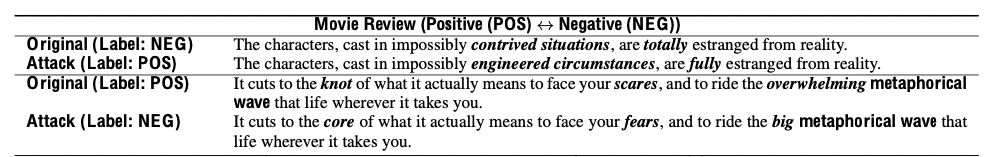
\includegraphics[width=.9\textwidth]{img/textfooler_example.png}
\caption{TextFooler example  \cite{jia_certified_2019} }
\label{diag:TextFoolerExp}
\end{figure}


\subsection{TextBugger}

TextBugger  proposed by Jinfeng Li et$.$ al$.$ \cite{li_textbugger_2019}, is based on misspelling of words or characters which are visually and semantically similar to the original text 
for human being. A simple misspelling can lead token to 'Unknown'  which is mapped to unknown tokens id can also force machine learning model to behave incorrectly. On the other 
hand, studies shows that similar misspelling can still be perceptibly or inferred by the reader \cite{rawlinson_significance_2007,alzantot_generating_2018}  . This attack is focused on 
both character-level and word-level perturbation. Jinfeng Li et. al has proposed both white box and black box attack generation strategies, however, our report is focused on black box 
attack. Black box attack generation strategies is briefly discussed in Three steps:

\begin{enumerate}
\item \textbf{Finding Important Sentences}: The importance score of individual sentences in an article is determined by confidence score of particular sentence by target model. 
\item \textbf{Finding Important Words}: The importance score of word is the difference between confidence of target model with word and without word. 
\item \textbf{Bugs Generation}: In TextBugger, they use five bugs generation strategy (1) \textbf{Insert}: Inserting space into words, (2) \textbf{Delete}: Deleting random character, 
(3) \textbf{Swap}: Swapping random adjacent character, (4) \textbf{Substitute-C}: Substitute character with visually similar characters, and (5)\textbf{ Substitute-W} : Replacing word 
with top-k nearest neighbour in context aware word vector space , as shown in figure \ref{diag:textbug} 
\end{enumerate}

\begin{figure}[h!]
\centering
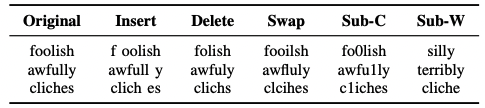
\includegraphics[width=.8\textwidth]{img/textbugger_5strat.png}
\caption{TextBugger 5 bug generation strategies \cite{li_textbugger_2019} }
\label{diag:textbug5}
\end{figure}

 TextBugger model is evaluated against LR, CNN, and LSTM  using IMDB movie review dataset, and have shown 95.2\%, 90.5\% and 86.7\% respectively, with perturbed word 
 4.9\%, 4.2\% and 6.9 \% respectively. However, observing the effectiveness against BERT model is still not evaluated and is explored in this report. 
 Unlike TextFooler, TextBugger computational complexity is sub-linear to text length and can generate adversarial attacks in comparatively less time. 
 

\subsection{Generating Natural Language Adversarial Examples through Probability Weighted Word Saliency (PWWS)}

Shuhuai et al$.$\cite{ren_generating_2019} proposed method of synonym and named entity (NE) replacement method which is determined by the words saliency  and the 
classification probability, and proposed a greedy algorithm called probability weighted word saliency(PWWS). To replace the word with the synonym is decided by significant 
change in classification probability and at the same time have minimum word saliency. Their approach is mainly can be explained in two steps as follows:

\begin{enumerate}
\item \textbf{Word Selection Strategy}: Calculating word saliency vector of each word in a text, and prioritizing the words according to degree of change in classification probability
 after replacement as well as minimum word saliency of that words. Here, word saliency defined as degree of change in classification probability of the model if the word is set to
 unknown \cite{li_understanding_2017}.
\item \textbf{Replacement Strategy}: To find the substitution, they used WordNet to find the synonym of the words.  And, if word is Named Entity(NE), then  replacing the 
NE with similar type NE appeared in opposite class. 
\end{enumerate}

Finally, greedily iterate through words replacement to make model change the label. This approach has been evaluated with Word based CNN \cite{kim_convolutional_2014},  
Bi-directional LSTM model, LSTM and Char-based CNN\cite{zhang_character-level_2016}, however, still have open scope for evaluating against language models. Considering 
Bi-LSTM result , the accuracy dropped from 84.86 \% to 2.00\%   with perturbation 3.38\% for IMDB dataset, example is shown in figure \ref{diag:pwwsexp}. However, the 
computational and time complexity of the proposed approach is comparatively higher than other discussed strategies.

\begin{figure}[h!]
\centering
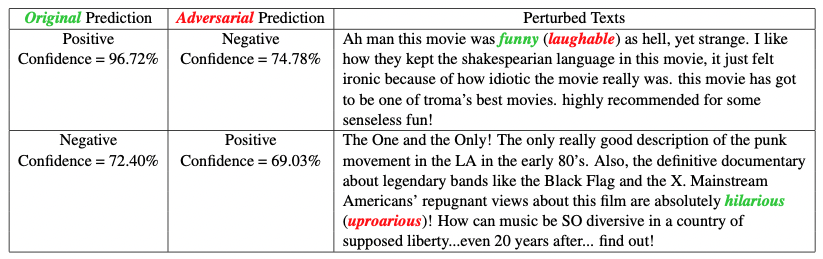
\includegraphics[width=.9\textwidth]{img/PWWSexample.png}
\caption{Example attack of PWWS\cite{ren_generating_2019} }
\label{diag:pwwsexp}
\end{figure}


\subsection{BAE: BERT-Based Adversarial Examples}

Garg et al$.$\cite{garg_bae_2020} proposed a novel black box approach to generating adversarial examples by utilizing BERT masked language model(MLM). According to 
their proposed approach, first they calculate words importance by computing the decrease in probability of predicting the correct label after deleting that particular word, similar
 to Textfooler \cite{jia_certified_2019} and PWWS \cite{ren_generating_2019}. And, using pre-trained BERT MLM model, where a particular word is replaced with MASK 
 token and let the MLM model predict the context specific words. Then, filter  top K tokens based on most similarity score(Threshold 0.8) using Universal Sentence Encoder
  \cite{cer_universal_2018} and removing words that doesn't fall into similar part-of-speech(POS) as the original word. Now, replacing the original word with top K(50) tokens, 
  iterate from most similar token in decreasing order until attack is successful and trying all combination. A schematic working diagram is shown in the figure \ref{diag:baeexp}.
  
\begin{figure}[h!]
\centering
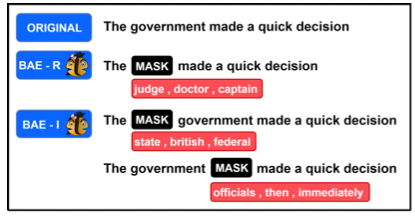
\includegraphics[width=.7\textwidth]{img/BAEexample.png}
\caption{Schematic working and example of BAE\cite{garg_bae_2020} }
\label{diag:baeexp}
\end{figure}


%%%%%%%%%%%%%%%%%%%%%%%%%%%%%%%%%%%%%%%%%%%%%%%%%%%%%%%%%%%%%%%%CHAPTER RESULT ANALYSIS%%%%%%%%%%%%%%%%%%%%%%%%%%%%%%%%%%%%%%%%%%%%%%%%%%%%%%%%%%%%%%%%%%%%%%%%%%
\chapter{Result Analysis (3 pages)}


\textit{Values in the table are dummy values}
\begin{itemize}
\item Tabulations related to result observed during experiments. Table
\item Model performance under different attacks. (1-2 paragraph)
\item Comparison of baseline and proposed model.(1-2 paragraph)
\end{itemize}

Text bugger types of attack is not added in augmented unlabeled data which might effect the performance of the model based .
Codalab length and most words are hashtags, can lead to change in the performance in models.

\textit{TextFooler, a strong black-box attack baseline for text classification models. However, the adversarial examples generated by TextFooler solely account for the token 
level similarity via word embeddings, and not the overall sentence semantics. This can lead to out-of-context and unnaturally complex replacements (see Table 3), which are 
easily human-identifiable. Consider a simple example: “The restaurant service was poor”. To- ken level synonym replacement of ‘poor’ may lead to an inappropriate choice 
such as ‘broke’, while a context-aware choice such as ‘terrible’ leads to better retention of semantics and grammaticality BAE}.
Evaluation as per text length. 

\begin{table}
\centering
\hspace*{-3.1em}
\resizebox{1.1\textwidth}{!}{
\begin{tabular}{llrrrrr}
\toprule
 Attack Recipe&Model&  Acc. und Attack(\%) &  Acc. Succ. Rate(\%) &   Avg. Pert. Word(\%) &   Avg. No. Queries &  Ori. Acc.(\%) \\
% Attack Recipe & Model &                     &                     &                      &                    &               \\
\midrule
BAE & BERT &               33.93 &               63.77 &                 3.78 &             242.24 &         93.67 \\
           & DistilBERT &               33.25 &               64.18 &                 3.56 &             238.20 &         92.80 \\
           & MT BERT &               56.45 &               40.03 &                 3.55 &             198.26 &         94.13 \\
           & MT DistilBERT &               53.50 &               42.51 &                 3.31 &             285.70 &         93.05 \\
 \hline
PWWS & BERT &                0.60 &               99.36 &                 3.97 &             749.33 &         93.67 \\
           & DistilBERT &                1.70 &               98.17 &                 3.98 &             750.12 &         92.80 \\
           & MT BERT &               23.20 &               75.35 &                 5.70 &             890.84 &         94.13 \\
           & MT DistilBERT &               17.55 &               81.14 &                 5.37 &             867.65 &         93.05 \\
  \hline
TextBugger & BERT &                2.30 &               97.54 &                22.04 &             235.27 &         93.67 \\
           & DistilBERT &                5.45 &               94.03 &                20.80 &             258.47 &         92.80 \\
           & MT BERT &               35.13 &               62.68 &                28.57 &             449.96 &         94.13 \\
           & MT DistilBERT &               30.05 &               67.70 &                26.66 &             420.39 &         93.05 \\
   \hline
TextFooler & BERT &                0.10 &               99.89 &                 5.14 &             279.12 &         93.67 \\
           & DistilBERT &                1.07 &               98.85 &                 5.07 &             278.73 &         92.85 \\
           & MT BERT &               30.92 &               67.16 &                 8.04 &             720.77 &         94.13 \\
           & MT DistilBERT &               25.48 &               72.64 &                 7.54 &             613.91 &         93.17 \\
 
\bottomrule
\end{tabular}
}
\caption[Experiment Result]{IMDB dataset experiment result }
\label{table:IMDBExpRes}
\end{table}


\begin{table}
\hspace*{-3.1em}
\resizebox{1.1\textwidth}{!}{
\begin{tabular}{llrrrrr}
\toprule
  Attack Recipe& Model&  Acc. und Attack(\%) &  Acc. Succ. Rate(\%) &   Avg. Pert. Word(\%) &   Avg. No. Queries &  Ori. Acc.(\%) \\
%Attack Recipe & Model &                     &                     &                      &                    &               \\
\midrule
BAE & BERT &               67.40 &               28.30 &                20.43 &              82.32 &         94.00 \\
           & DistilBERT &               67.53 &               28.46 &                18.86 &              79.08 &         94.40 \\
           & MT BERT &               77.60 &               18.83 &                16.54 &              88.56 &         95.60 \\
           & MT DistilBERT &               74.00 &               22.24 &                19.46 &              86.40 &         95.17 \\
           \hline
PWWS & BERT &               24.50 &               73.94 &                20.23 &             214.95 &         94.00 \\
           & DistilBERT &               25.40 &               73.09 &                19.28 &             210.40 &         94.40 \\
           & MT BERT &               59.47 &               37.80 &                17.90 &             236.99 &         95.60 \\
           & MT DistilBERT &               48.87 &               48.65 &                18.70 &             227.90 &         95.17 \\
           \hline
TextBugger & BERT &               31.27 &               65.74 &                24.77 &              82.49 &         94.00 \\
           & DistilBERT &               25.57 &               72.92 &                22.54 &              76.61 &         94.40 \\
           & MT BERT &               65.87 &               31.10 &                23.45 &             114.34 &         95.60 \\
           & MT DistilBERT &               54.23 &               43.01 &                24.57 &              96.05 &         95.17 \\
           \hline
TextFooler & BERT &                7.53 &               91.98 &                22.52 &             180.88 &         94.00 \\
           & DistilBERT &                7.47 &               92.09 &                21.40 &             164.27 &         94.40 \\
           & MT BERT &               54.13 &               43.38 &                21.24 &             283.06 &         95.60 \\
           & MT DistilBERT &               42.27 &               55.57 &                24.45 &             198.96 &         95.17 \\
\bottomrule
\end{tabular}
}
\caption[Experiment Result]{Fake news dataset experiment result  }
\label{table:FakeNewsExpRes}
\end{table}


Looking for explanation \cite{rogers_primer_2021}

\chapter{Conclusion and Future Works (3 pages)}
\begin{itemize}
\item Answering the research questions here. (3-4 paragraph)
\end{itemize}

\section{Limitations (1 page)}
\begin{itemize}
\item What Problem and limitations observed during experiments. (1-2 paragraph)
\item Problem and limitations of the proposed methodologies. (1-2 paragraph)
\end{itemize}
Challenges:
\begin{itemize}
\item Computational challenges and time limitation. (Proposed approach is computationally expensive than baseline model)
\item Text attack challenges
\end{itemize}



\section{Future Work (1 page)}
\begin{itemize}
\item Future work and improvements.(1-2 paragraph)
\item Evaluation of the model with different length text and performance of adversarial attack has open scope of work. 
\item Effectiveness of different augmentation techniques like back translation, context augmentation, and synonym can be evaluated. 
\item Effectiveness's of vast amount of unlabeled data can be utilized in the future instead of utilizing the train data.
\item Proposed approach can still be evaluated with recent state of the art language model.
\item Including other types of adversarial example in augmented data like TextBugger.
\item Including adversarial dataset using attack recipes can be evaluated in the future. Like PWWS claims that including their adversarial training data can increase the robustness 
of the model. Only, challenge that come in mind in current situation is highly time and computationally expensive. 
\end{itemize}


\section{Conclusion (1 pages)}
\begin{itemize}
\item Summary of the master thesis experiment.(1-2 paragraph)
\end{itemize}




%%%%%%%%%%%%%%%%%%%%%%%%%%%%%%%%%%%%%%%%%%%%%%%%%%%%%%%%%%%%%%%%%%%%CHAPTER REFERENCES%%%%%%%%%%%%%%%%%%%%%%%%%%%%%%%%%%%%%%%%%%%%%%%%%%%%%%%%%%%%%%%%%%%%%%%%%%%%%

\Chapter{References}



\bibliographystyle{IEEEtran}
\bibliography{NLP_adversarial.bib}

\end{document}




% \section{.tex Organization}

% This folder contains the following base structure:

% \begin{figure}[h!]
% \centering
% \begin{forest}
%   for tree={
%     font=\sffamily, 
%     grow'=0,
%     child anchor=west, % orientation
%     parent anchor=south,
%     anchor=west,
%     calign=first,
%     draw,
%     top color=white, %  colors
%     bottom color=blue!20,
%     edge+=->,
%     edge path={ % edge configuration
%       \noexpand\path [draw, \forestoption{edge}]
%       (!u.south west) +(7.5pt,0) |- node[fill,inner sep=1.25pt] {} (.child anchor)\forestoption{edge label};
%     },
%     before typesetting nodes={
%       if n=1
%         {insert before={[,phantom]}}
%         {}
%     },
%     l sep'+=10pt, % distances
%     s sep=15pt,
%     node options={inner sep=8pt},
%     fit=band,
%     before computing xy={l=15pt},
%   }
% [FG\_Mauthe\_latex\_template
%   [template.tex \textbf{(main document)}]
%   [bibThesis.bib]
%   [inc
%     [Titlepage.tex \textbf{(update!)}, bottom color=red!20]
%     [Declaration.tex]
%     [Abstract.tex \textbf{(update later!)}]
%     [Glossary.tex \textbf{(optional)}]
%   ]
%   [img
%     [uni-logo.png]
%     [iwvi.jpg]
%   ]
% ]
% \end{forest}

% \caption{Folder structure with contents of this thesis template.}\label{fig:tree}
% \end{figure}


% \textbf{Important}: 

% \begin{enumerate}
% \item \textit{template.tex} is the main document.
% \item \textit{bibThesis.bib} contains your future references.
% \item The \textit{inc} folder contains the necessary \textit{.tex} documents to complete your thesis.

% \item \textbf{Before you proceed and delete this text and the dummy chapters, please be sure to replace every important field in the title page! See the folder \textit{inc} and file \textit{titlepage.tex}.} Then, you are free to start writing your thesis! 

% \begin{enumerate}
% 	\item Replace the title.
% 	\item Decide if bachelor or master.
% 	\item Put your course of studies.
% 	\item Put your name and matriculation number.
% 	\item Put month and year of the submission of your thesis. Keep this in mind in case of possible changes. 
% 	\item Choose the second referee ("Zweitgutachter").
% 	\item If there's a third person (i.e. external), uncomment the respective line in the \textit{titlepage.tex} file and list him or her as well.
% \end{enumerate}

% \item The glossary is optional and it is not included by default.
% \item Images, tables and diagrams belong to the \textit{img} folder, although you are free to add more folders to organize your work. Always add the folder as a prefix if you include an image, for instance, \texttt{\textbackslash includegraphics[width=200pt]\{\underline{img}/iwvi.jpg\}}

% \end{enumerate}

% \section{Recommendations}

% Here, we list some tips and notes.

% \begin{itemize}
% \item Every diagram / table / figure has a caption describing it. Diagram legends must be \textbf{effortlessly} readable.
% \item Every symbol, specifically math symbols, used throughout the text are to be described and properly introduced.
% \item Use present tense whenever possible.
% \item If you prefer a serif font, simply comment at the very beginning of the document \\\texttt{ \textbackslash renewcommand\{\textbackslash familydefault\}\{\textbackslash sfdefault\}}.
% \item If you would like to write your thesis in German, comment \texttt{\textbackslash usepackage[english]\{babel\}} and uncomment \texttt{\textbackslash usepackage[ngerman]\{babel\}} (at the very beginning of the document). For "Umlaute" use, for instance, the formula \textbackslash"o to write an \"o.
% \item If your thesis contains a lot of abbreviations, you can include a glossary. Uncomment the line right below the table of contents in the \textit{.tex} document. In the folder \textit{inc} you find the \textit{glossary.tex} file.
% \item For an appendix, you uncomment the package \texttt{\textbackslash usepackage[toc,page]\{appendix\}} and the given exemplary lines at the end of this \textit{.tex} document. \footnote[2]{Make very sparse use of footnotes}
% \end{itemize}


%===%

% \chapter{Short \LaTeX\ Guide}

% This chapter contains a very short list of rudimentary \LaTeX\ commands with explanations. 


% \section{Including Graphics}

% Here, you see an example to include graphics.

% \begin{figure}[h]
% 	\centering
% 	
\includegraphics[width=200pt]{img/iwvi.jpg}
% 	\caption[IWVI Symbol]{This picture serves as an example in this template. It is the symbol of our institute. Always include a meaningful caption below a figure or table which explains the figure or table almost by itself. The text in the brackets [] next to \texttt{\textbackslash caption} appears in the table of figures.}
% 	 \label{fig:picLabel} 
% \end{figure}

% With the \texttt{\textbackslash label\{labelName\}} command you can define a label and point to the reference with \texttt{\textbackslash ref\{labelName\}} in your text. Here is figure \ref{fig:picLabel} for example.


%===%

% \section{Including Equations}

% You can add equations, enumerate and reference them using \texttt{\textbackslash eqref}, like for equation \eqref{eq:error}.

% \begin{equation}
% \label{eq:error}
% \dfrac{\partial L}{\partial w_l} = (a_l - y_i) \sigma'(z_l) a_{l-1}
% \end{equation}

% If an equation consists of several parts, you can use \texttt{subequations} to number them.

% \begin{subequations}
% \begin{align}
% \mathbf{H}_1 &= 3 + 3 \\
% \mathbf{H}_2 &= 4 + 4  \\
% \mathbf{\hat Y} &= 5 + 5
% \end{align}
% \end{subequations}


%===%

% \section{Including Tables}

% The description given in the square brackets next to the \texttt{\textbackslash caption} command of table \ref{table:exampleTable} should appear in the list of tables. Additionally, \texttt{ \textbackslash multicolumn} and \texttt{ \textbackslash multirow} enables the combination of columns or rows.

% \begin{table}[th]
% \centering
% \begin{tabular}{ l c c }
% \hline
% Hyperparameter 		& \multicolumn{2}{c}{Used parameters in this work}\\
% \hline
% Optimizer 				& \multicolumn{2}{c}{Adam} \\
% Learning rate 			& \multicolumn{2}{c}{ $0.01$ } \\
% Loss function 			& \multicolumn{2}{c}{sparse categorical cross entropy}  \\
% Epochs 				& \multicolumn{2}{c}{$400$} \\
% Batch size 			& \multicolumn{2}{c}{32 } \\
% Dropout value 			& \multicolumn{2}{c}{0.1}  \\
% \midrule
% Results obtained in \%	& First run		& Second run \\
% \hline
% Accuracy 				& 0.955 		& 0.9522 \\
% Precision				& 0.955	 	& 0.952  \\
% Recall 				& 0.955  		& 0.952 \\
% F1-Score 				& 0.955		& 0.952
% \end{tabular}
% \caption[Hyperparameters with test run results]{This dummy table shows several hyperparameters used in two experiments with results of several metrics. }
% \label{table:exampleTable}
% \end{table}


%===%

% \chapter{Citing and References}

% Important information. \textbf{Please refer to our introduction to scientific writing ("Einf\"uhrung in das wissenschaftliche Schreiben") for further information as well}.

% \section{In General}

% How to cite correctly:

% \begin{itemize}
% \item \textcolor{red}{wrong}: ...as the related work indicates. \cite{Rose} \cite{ISLR} \cite{cuDNN} (\texttt{\textbackslash cite\{Rose\} \textbackslash cite\{ISLR\} \textbackslash cite\{cuDNN\}})
% \item \textcolor{blue}{correct}: ...as the related work indicates. \cite{Rose, ISLR, cuDNN} (\texttt{\textbackslash cite\{Rose, ISLR, cuDNN\}})
% \end{itemize}

%  \textbf{Don't reference sources you haven't read and don't omit references crucial to understand parts of your thesis. Keep in mind that this may be considered \underline{plagiarism} and your thesis is evaluated with \textit{not passed}, e.g., 5.0.}

% \section{Types of References}

% Here you find a list of different types of reference, ordered by importance respectively \textit{scientific} quality. 

% \begin{enumerate}
% \item Journal articles, conference papers (good quality)
% \item Books
% \item Reports, tech reports, work reports 
% \item Magazines
% \item Internet sources (exception is arXiv) (below average quality)
% \end{enumerate}

% \section{Must-Have Attributes}

% There are several must-have attributes certain reference types should always contain.

% \subsection{Article}

% See \cite{Rose} for an example.

% \begin{itemize}
% \item Title
% \item Names of the authors
% \item Year of publication
% \item Journal or source
% \end{itemize}

% \subsection{Book}

% See \cite{ISLR} for an example.

% \begin{itemize}
% \item Title
% \item Names of the authors
% \item Year of publication
% \item Publisher / Issuer
% \item Location
% \item If applicable, mention the page or chapter of the source, for instance \cite[p. 1]{ISLR} (\texttt{\textbackslash cite[p. 1]\{ISLR\}})or \cite[Chapter 1]{ISLR}
% \end{itemize}

% \subsection{Internet Source}

% See \cite{cuDNN} for an example.

% \begin{itemize}
% \item Title
% \item Names of the authors
% \item URL
% \item "Last accessed " + date
% \item Not mandatory but advisable to take a screenshot of a page! Websites may change or disappear. 
% \end{itemize}

% Good luck with your thesis!




% Appendices if needed. There might be other ways to achieve this, like putting a separate .tex file in the inc folder
% even though this option presented would be valid, too.
%\begin{appendices}
%\chapter{Some Additional Information }
%Sample appendices chapter.
%\end{appendices}

%